\documentclass[a4paper,12pt]{article}
\usepackage{graphicx}
\usepackage[backend=biber]{biblatex}
\usepackage{float}
\usepackage[swedish]{babel}
\usepackage{pdfpages} 
\usepackage[titletoc]{appendix}
\addbibresource{bibliography.bib}
%% Definitioner f�r LIPS-dokument

\usepackage[utf8]{inputenc}
\usepackage[swedish]{babel}
\usepackage[T1]{fontenc}
\usepackage{times}
\usepackage{ifthen}

\usepackage[margin=25mm]{geometry}

\usepackage{fancyhdr}
\pagestyle{fancy}
\lhead{}
\chead{\textbf{\LIPSprojekttitel}}
\rhead{\textbf{\LIPSdatum}}
\lfoot{\textbf{\LIPSkursnamn}\\\textbf{LIPS Slutrapport}}
\cfoot{\textbf{\thepage}\\\textbf{\LIPSgruppepost}}
\rfoot{\textbf{\LIPSprojektgrupp}}

\setlength{\parindent}{0pt}
\setlength{\parskip}{1ex plus 0.5ex minus 0.2ex}


\newcommand{\twodigit}[1]{\ifthenelse{#1<10}{0}{}{#1}}
\newcommand{\dagensdatum}{\number\year-\twodigit{\number\month}-\twodigit{\number\day}}

%%  Redefinitions of commands containing @
\makeatletter
\makeatother

\newcommand{\LIPStitelsida}{%
{\ }\vspace{45mm}
\begin{center}
  \textbf{\Huge \LIPSdokumenttyp}
\end{center}
\begin{center}
  {\Large Redaktör: \LIPSredaktor}
\end{center}
\begin{center}
  {\Large \textbf{Version \LIPSversion}}
\end{center}
\vfill
\begin{center}
  {\large Status}\\[1.5ex]
  \begin{tabular}{|*{3}{p{40mm}|}}
    \hline
    Granskad & \LIPSgranskare & \LIPSgranskatdatum \\
    \hline
    Godkänd & \LIPSgodkannare & \LIPSgodkantdatum \\
    \hline
  \end{tabular}
\end{center}
\newpage
}


\newenvironment{LIPSprojektidentitet}{%
{\ }\vspace{45mm}
\begin{center}
  {\Large PROJEKTIDENTITET}\\[0.5ex]
  {\small
  \LIPSartaltermin, \LIPSprojektgrupp\\
  Linköpings Tekniska Högskola, IFM
  }
\end{center}
\begin{center}
  {\small Gruppdeltagare}\\
%  \begin{tabular}{|p{30mm}|p{40mm}|p{35mm}|p{45mm}|}
  \begin{tabular}{|l|l|p{25mm}|l|}
    \hline
    \textbf{Namn} & \textbf{Ansvar} & \textbf{Telefon} & \textbf{E-post} \\
    \hline
}%
{%
    \hline
  \end{tabular}
\end{center}
\begin{center}
  {\small
    %\textbf{E-postlista för hela gruppen}: \LIPSgruppepost\\
    %\textbf{Hemsida}: \LIPSgrupphemsida\\[1ex]
    \textbf{Kund}: \LIPSkund\\
    \textbf{Kontaktperson hos kund}: \LIPSkundkontakt\\
    \textbf{Kursansvarig}: \LIPSkursansvarig\\
    \textbf{Handledare}: \LIPShandledare\\
  }
\end{center}
\newpage
}
\newcommand{\LIPSgruppmedlem}[4]{\hline {#1} & {#2} & {#3} & {#4} \\}



\newenvironment{LIPSdokumenthistorik}{%
\begin{center}
  Dokumenthistorik\\[1ex]
  \begin{small}
    \begin{tabular}{|l|l|p{60mm}|l|l|}
      \hline
      \textbf{Version} & \textbf{Datum} & \textbf{Utförda förändringar} & \textbf{Utförda av} & \textbf{Granskad} \\
      }%
    {%
      \hline
    \end{tabular}
  \end{small}
\end{center}
}
\newcommand{\LIPSversionsinfo}[5]{\hline {#1} & {#2} & {#3} & {#4} & {#5} \\}

\newcounter{LIPSkravnummer}
\newcounter{LIPSunderkravnummer}[LIPSkravnummer]
\newenvironment{LIPSkravlista}{%
  \begin{tabular}{|p{25mm}|p{25mm}|p{72mm}|p{18mm}|}
    }%
  {%
    \hline
  \end{tabular}
}
\newcommand{\LIPSkrav}[3]{\hline\stepcounter{LIPSkravnummer}\textbf{Krav nr \arabic{LIPSkravnummer}} & \textbf{{#1}} & {#2} & \textbf{{#3}} \\}
\newcommand{\LIPSunderkrav}[3]{\hline\stepcounter{LIPSunderkravnummer}\textbf{Krav nr \arabic{LIPSkravnummer}\Alph{LIPSunderkravnummer}} & \textbf{{#1}} & {#2} & \textbf{{#3}} \\}

\newcounter{LIPSMilstolpar}
\newenvironment{LIPSMilstolpslista}{%
  \begin{tabular}{|p{15mm}|p{72mm}|p{25mm}|}
\hline
\textbf{Nr} & \textbf{Beskrivning} & \textbf{Datum} \\
    }%
  {%
  \hline
  \end{tabular}
}
\newcommand{\LIPSMilstolpar}[2]{\hline\stepcounter{LIPSMilstolpar}\textbf{ \arabic{LIPSMilstolpar}.} & \textbf{{#1}} & \textbf{{#2}} \\}

\newcounter{LIPSBeslutspunkter}
\newenvironment{LIPSBeslutspunktslista}{%
  \begin{tabular}{|p{15mm}|p{72mm}|p{25mm}|}
\hline
\textbf{Nr} & \textbf{Beskrivning} & \textbf{Datum} \\
    }%
  {%
  \hline
  \end{tabular}
}
\setcounter{LIPSBeslutspunkter}{-1}
\newcommand{\LIPSBeslutspunkter}[2]{\hline\stepcounter{LIPSBeslutspunkter}\textbf{ \arabic{LIPSBeslutspunkter}.} & \textbf{{#1}} & \textbf{{#2}} \\}

\newcounter{LIPSAktiviteter}
\newenvironment{LIPSAktivitetslista}{%
  \begin{tabular}{|p{15mm}|p{72mm}|p{25mm}|}
\hline
\textbf{Nr} & \textbf{Beskrivning} & \textbf{Datum} \\
    }%
  {%
  \hline
  \end{tabular}
}
\newcommand{\LIPSAktiviteter}[2]{\hline\stepcounter{LIPSAktiviteter}\textbf{ \arabic{LIPSAktiviteter}.} & \textbf{{#1}} & \textbf{{#2}} \\}




%%% Local Variables: 
%%% mode: latex
%%% TeX-master: "kravspec_mall"
%%% End: 
\pagenumbering{roman}
\newcommand{\LIPSartaltermin}{2018/VT}
\newcommand{\LIPSkursnamn}{TFYA75}

\newcommand{\LIPSprojekttitel}{Visualisering av elektronstruktur}

\newcommand{\LIPSprojektgrupp}{Grupp 2}
\newcommand{\LIPSgruppepost}{}
\newcommand{\LIPSdokumentansvarig}{Marian Brännvall}

\newcommand{\LIPSkund}{IFM, Linköpings universitet, 581\,83 Linköping}
\newcommand{\LIPSkundkontakt}{Rickard Armiento, 013-281249, rickard.armiento@liu.se}
\newcommand{\LIPSkursansvarig}{Per Sandström, 013-282902, persa@ifm.liu.se}
\newcommand{\LIPShandledare}{Johan Jönsson, 013-281176, johan.jonsson@liu.se}


\newcommand{\LIPSdokumenttyp}{Kappa}
\newcommand{\LIPSredaktor}{Anders Rehult}
\newcommand{\LIPSversion}{xx}
\newcommand{\LIPSdatum}{\dagensdatum}

\newcommand{\LIPSgranskare}{DOK}
\newcommand{\LIPSgranskatdatum}{18-03-05}
\newcommand{\LIPSgodkannare}{}
\newcommand{\LIPSgodkantdatum}{}

\usepackage[titletoc]{appendix}
\usepackage{hyperref}
\hypersetup{
    colorlinks,
    citecolor=black,
    filecolor=black,
    linkcolor=black,
    urlcolor=black
}

\begin{document}

\LIPStitelsida

%Får väldigt gärna omformuleras och utökas
%Ska man tacka Per?
\subsection*{Förord}
%\addcontentsline{toc}{subsection}{Förord}
Vi vill rikta ett stort tack till vår handledare Johan Jönsson som varit ett viktigt stöd under arbetets gång. Vi vill även tacka vår beställare Rickard Armiento som vi också har kunnat vända oss till med frågor.
\newpage


\begin{abstract}
% Kan behöva omformuleras!
Det är viktigt att kunna göra olika typer av visualiseringar baserat på elektronstrukturberäkningar, detta för att bland annat kunna presentera resultat från forskning inom materialfysik på ett enklare sätt. Detta dokument är en kappa för slutrapporten för kandidatprojektet i visualisering av elektronstrukturer. Kappan beskriver bland annat projektets problemformulering och resultat, dessutom finns en beskrivning av genomförandet av projektet samt en teknisk beskrivning av det visualiseringsverktyget som tagits fram.
\newpage
\end{abstract}

\begin{LIPSprojektidentitet}
  \LIPSgruppmedlem{Anders Rehult}{Projektledare (PL)}{076-3161206}{andre449@student.liu.se}
  \LIPSgruppmedlem{\LIPSdokumentansvarig}{Dokumentansvarig (DOK)}{070-7280044}{marbr639@student.liu.se}
  \LIPSgruppmedlem{Andreas Kempe}{Sekreterare (SE)}{073-9796689}{andke133@student.liu.se}
  \LIPSgruppmedlem{Viktor Bernholtz}{Viktor Bernholtz (VB)}{073-0386030}{vikbe253@student.liu.se}
\end{LIPSprojektidentitet}

\tableofcontents{}
\newpage

\addcontentsline{toc}{section}{Dokumenthistorik}
\begin{LIPSdokumenthistorik}
  \LIPSversionsinfo{0.1}{2018-}{Första utkast.}{Projektgruppen}{}
\end{LIPSdokumenthistorik}
\newpage
\pagenumbering{arabic}

\section{Inledning}
\label{ch:inledning}
Dokumentet är en kappa för slutrapporten för kandidatprojektet i visualisering av elektronstrukturer. Visualisering av elektronstrukturer är ett av projekten i kursen TFYA75 vid
Linköpings universitet. 

Inom materialfysik är elektronstrukturberäkningar ett viktigt teoretiskt verktyg. Detta för att få en så bra förståelse som möjligt av hur olika material är uppbyggda, bland annat vad gäller kristallers egenskaper sett ur ett kvantmekaniskt perspektiv. Det kan exempelvis handla om att man vill ta reda på olika materials egenskaper vad gäller värmeledningsförmåga, strömledningsförmåga etc.

För att öka förståelsen samt för att enklare kunna presentera resultat från forskning inom området är det viktigt att kunna göra olika typer av visualiseringar baserat på elektronstrukturberäkningar.

I många av de system som används för att utföra dessa beräkningar, exempelvis VASP, ges ingen eller begränsad möjlighet till detta. Vidare är de system som idag finns tillgängliga för visualisering förhållandevis ineffektiva, dåligt standardiserade samt har få visualiseringsfunktioner.

Projektgruppen har vidareutvecklat och utökat det system som togs fram av 2017 års projektgrupp. Utöver det konkreta målet med utvecklingen av mjukvara för visualisering ska även projektet ge projektmedlemmarna erfarenhet av att arbeta i projekt och utöka deras förmåga till analytiskt och fysikaliskt tänkande för att ge värdefull erfarenhet inför arbetslivet.

Kappan ger en översikt över hela projektet och består av följande delar:

\begin{itemize}
	\item \textbf{Problemformulering}, avsnitt \ref{ch:problemformulering} och \textbf{Kunskapsbas}, avsnitt \ref{ch:kunskapsbas}, beskriver själva förarbetet i projektet.
	
	\item \textbf{Fördjupningsarbeten}, se avsnitt \ref{ch:fördjupningsarbeten} beskriver kortfattat de fördjupningsområden som projektgruppen behandlat.
	
	\item \textbf{Fasplan}, avsnitt \ref{ch:fasplan} beskriver överskådligt hur projektet har genomförts.

	\item \textbf{Teknisk beskrivning}, avsnitt \ref{ch:teknisk-beskrivning} beskriver överskådligt hur systemet är uppbyggt.
	
	\item \textbf{Resultat}, avsnitt \ref{ch:resultat} och \textbf{Slutsats}, avsnitt \ref{ch:slutsats} beskriver vilka krav som är uppfyllda och hur det slutgiltiga resultatet blev samt sammanfattar projektet i sen helhet.
\end{itemize}

% TODO: Ska parter, användning och begränsningar vara med?
\subsection{Parter}
Rickard Armiento har beställt systemet som är beskrivet i kappan. Medlemmarna i projektgruppen, som är listade under rubriken projektidentitet ovan, är mottagare av denna beställning och har haft i uppgift att implementera systemet. Projektgruppens handledare är Johan Jönsson.


\subsection{Användning}
Denna produkt kommer användas vid Linköpings universitet för att analysera data från elektronstruktursberäkningar.

\subsection{Begränsningar}
I projektet har visualiseringsverktyget Inviwo och
programmeringspråken Python och C++ användts. Det har inte utretts
om det är bättre att använda andra verktyg.

\subsection{Definitioner}

\textbf{C++} är ett programmeringsspråk.
\cite{C++}
\newline
I Inviwo används C++ för att skriva programkod till
processorer.

\textbf{Fermi-yta} är, för elektroners k-punkter i reciproka rymden, isoytan där elektronernas energi är lika med Fermi-energin.
\cite{Fermi-yta}

\textbf{HDF5} är ett filformat som kan hantera stora mängder data.
\cite{hdf5}

\textbf{Inviwo} (Interactive Visualization Workshop) är programvara
för visualisering som tillhandahåller en nätverksredigerare för
designen av dataflödesnätverk. Noderna i dessa dataflödesnätverk
kallas processorer. Indata till nätverket behandlas i dessa
processorer och utdata genereras.
\cite{Inviwo}

\textbf{Python} är ett programmeringsspråk.
\cite{Python}
\newline
I Inviwo används Python för att knyta samman processorer.


\section{Problemformulering}
\label{ch:problemformulering}

I projektdirektivet, se appendix \ref{appendix:projektdirektiv}, ges en översiktlig bild av de krav som kan komma att ställas på systemet. Utifrån projektdirektivet har projektgruppen skapat en kravspecifikation, se appendix \ref{appendix:kravspecifikation} med de krav som ställs på sytemet och även de generella krav som ställs på projektet och dokumentationen.

Systemet ska vara ett verktyg för att visualiserar olika egenskaper från elektonstrukturberäkningar och själva visualiseringen ska ske i programvaran Inviwo\cite{Inviwo}.
Systemet ska vara uppbyggt av två huvudsakliga delsystem, ett som hanterar konvertering av data och ett annat som visualiserar den konverterade datan, se figur \ref{fig:grov-skiss}. Vilken data som ska visualiseras ska kunna väljas av användaren. Systemet ska vara en vidareutveckling av det system som togs fram av 2017 års projektgrupp. Projektegruppen ska utöka och uppdatera befintlig kod för att uppfylla de krav som ställts i kravspecifikationen.

\begin{figure}[H]
	\centering
	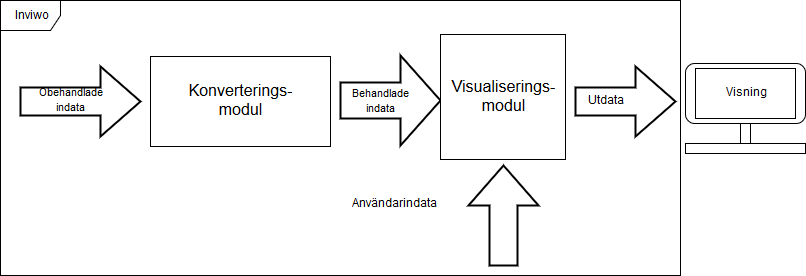
\includegraphics[scale=0.55]{grov-skiss.png}
	\caption{Grov design av systemet}
	\label{fig:grov-skiss}
\end{figure}



\section{Kunskapsbas}
\label{ch:kunskapsbas}
Projektgruppen har efter att ha tagit del av projektdirektivet, se appendix \ref{appendix:projektdirektiv},
skrivit en kravspecifikation, se appendix \ref{appendix:kravspecifikation}. Därefter skrevs en projektplan, se appendix \ref{appendix:projektplan}, tidplan, se appendix \ref{appendix:tidplan} och en  systemskiss, se appendix \ref{appendix:systemskiss} enligt LIPS-modellen \cite{LIPS}. 
% TODO: Fixa ref för LIPS
Dessa dokument har sedan fungerat som en utgångspunkt för projektets utforming. Utöver dessa har en designspecifikation, se appendix \ref{appendix:designspecifikation} skrivits som är en fördjupning i systemskissen och ger en mer detaljerad beskrivning av systemet.

Projektgruppen har skrivit två fördjupningsarbeten, se appendix \ref{appendix:fermi-ytor} och \ref{appendix:visualisering} knutna till projektarbetet.

Projektgruppen har tagit del av ett antal föreläsningar om dokumentationen i projektet. Utöver det har även föreläsningar i Inviwo och Python hållts samt laborationer i beräkningsfysik och Python-programmering. 

\section{Fasplan}
\label{ch:fasplan}
Projektet drivs enligt LIPS-modellen, som är en modell med regler, instruktioner och mallar för att bedriva projekt. Projektet delas upp i tre faser - före, under, och efter.

\subsection{Före-fas}
Före-fasen är ämnad att undersöka om projektet bör genomföras och, om så är fallet, definiera och konkretisera projektets mål samt organisera arbetet som krävs för att uppnå dessa. Under före-fasen skrivs bland annat ett projektdirektiv, se appendix \ref{appendix:projektdirektiv}, en kravspecifikation, se appendix \ref{appendix:kravspecifikation}, en systemskiss, se appendix \ref{appendix:systemskiss} och en projektplan, se appendix \ref{appendix:projektplan}. Projektdirektivet skrevs innan projektgruppen skapades och gavs till projektgruppen vid projektets start.
Projektgruppen har under före-fasen skrivit ett gruppkontrakt, se appendix \ref{appendix:Gruppkontrakt}, en kravspecifikation, en systemskiss samt en projektplan.

\subsection{Under-fas}
Under  under-fasen  utförs  det  arbete  som  leder  till  att  projektets  krav  uppfylls.  Projektgrup-
pen skriver en designspecifikation, se appendix \ref{appendix:designspecifikation}
som beskriver hur systemet ska konstrueras i mer detalj än
systemskissen. Projektgruppen arbetar sedan med att, utgående från denna designspecifikation, konstruera och testa systemet. En teknisk dokumentation, se appendix \ref{appendix:teknisk-dokumentation}, skrivs parallellt med systemets konstruktion för att reflektera den faktiska implementationen av idéerna beskrivna i designspecifikationen. 

Projektgruppen har också skrivit två fördjupningsarbeten knutna till projektet. Det ena, se appendix \ref{appendix:fermi-ytor}, behandlar Fermi-ytor som är ett av fördjupningsområdena i projektet och som ska visualiseras. Det andra, se appendix \ref{appendix:visualisering}, behandlar visualisering som är en mer generell del av projektet. 

\subsection{Efter-fas}
Under efter-fasen överförs projektresultatet till beställaren och projektet avslutas. Projektgruppen skriver en kappa som bifogas vid slutleveransen av produkten och även en användarmanual, se appendix \ref{appendix:användarmanual}. Vid slutleveransen ska
även en demonstration hållas som visar att produkten uppfyller kraven ställda på den. Efter produkten levererats skriver projektgruppen en efterstudie.

\section{Fördjupningsarbeten}
\label{ch:fördjupningsarbeten}
Nedan beskrivs kortfattat de fördjupningsarbeten som gjorts under projektet. Dessa finns även i sin helhet i appendix \ref{appendix:fermi-ytor} och \ref{appendix:visualisering}. 
\subsection{Fermi-ytor}
Syftet med fördjupningsarbetet om Fermi-ytor var att besvara följande frågor: Vad är Fermi-ytor och hur kan dessa beräknas numeriskt? Detta var av intresse för projektet eftersom en del av det bestod i att visualisera Fermi-ytor. Arbetet beskriver kortfattat begrepp inom fasta tillståndets fysik som är av betydelse för att förstå vad Fermi-ytor är, för att sedan gå in på hur dessa kan beräknas numeriskt.

\subsection{Visualisering av volymdata}
I fördjupningsarbetet, visualisering av volymsdata tittades det närmare på ett par av de metoder mjukvaran Inviwo använder sig av. Detta för att kunna göra en jämförelse av både prestanda och resultat.
\section{Teknisk beskrivning}
\label{ch:teknisk-beskrivning}

% TODO: En beskrivning av det  färdigställda systemet kan ses i figur. lägg till fig
Systemet hanterar indata från VASP.Datan kommer från elektronstrukturberäkningar och konverteras till HDF5-format för att därefter visualiseras. Användaren kan välja vad som ska visualiseras, kontrollera renderingens utseende och ställa in egenskaper såsom färg, transparens och rotation.
Systemet har delats in i delsystem och dessa har utvecklas och testas enskilt i den mån det inte funnits beroenden till andra delsystem.

I avsnitt \ref{ch:datakonvertering} och \ref{ch:visualisering} nedan ges en övergripande inblick i det två stora delsystemen och deras delsystem. För en mer detaljerad teknisk beskriving av systemet se den tekniska dokumentationen, se appendix \ref{appendix:teknisk-dokumentation}.

\subsection{Datakonvertering}
\label{ch:datakonvertering}
Detta avsnitt behandlar delsystemet datakonvertering, figur \ref{fig:konverteringdetalj} ger en grov översikt av delsystemet. Obehandlad data skickas in där obehandlad data är i form av textfiler med data från beräkningar gjorda i VASP. Indata behandlas sedan i konverteringsmodulen. Från konverteringsmodulen kommer behandlad data i HDF5-format.

\begin{figure}[H]
	\centering
	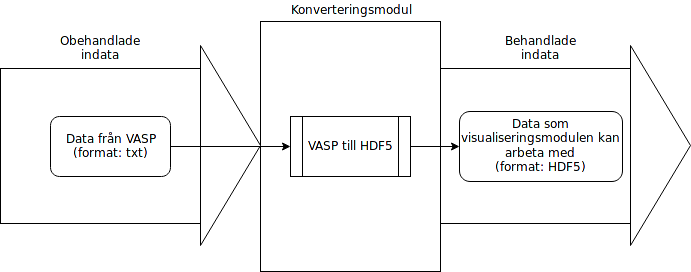
\includegraphics[scale=0.55]{konverteringdetalj.png}
	\caption{Grov design av konverteringsmodulen}
	\label{fig:konverteringdetalj}
\end{figure}

\subsubsection{HDF5}
Systemet kan hantera de olika utdatafilerna från VASP. Detta görs genom att konvertera datan till HDF5-format.
HDF5 är ett filformat som är designat för att hantera stora mängder data på ett flexibelt sätt \cite{hdf5}.
HDF5 har flera olika datatyper, se Figur 3, och ett HDF5-objekt som antingen är lagrat på disk eller hålls i minnet är uppdelat i två huvudsakliga underobjekt, nämligen grupper och dataset.
%ref[8, s. 3-4]

Alla HDF5-objekt har en rotgrupp som äger alla andra objekt i datastrukturen. Denna grupp innehåller i sin tur all övrig data i form av andra grupper, länkar till andra grupper eller dataset.
Dataset innehåller rådata av något slag. Rådata kan i sammanhanget vara bilder, utdata från beräkningar, programdata, etc. %ref [8, s. 4-5]
I desingspesifikationen, se appendix \ref{appendix:designspecifikation} ges en mer detaljerad beskriving av HDF5.

\subsubsection{VASP}
Från beräkningsprogrammet VASP fås en rad olika utdatafiler. Dessa listas och beskrivs i designspecifikationen 
(se appendix \ref{appendix:designspecifikation}). Ur dessa utdatafiler läses saker som atompositionsdata, gittervektorer, elektrontäthetsdata, tillståndstäthetsdata, Fermi-energi och så vidare för att kunna visualisera kristallstrukturer, elektrontäthet, ELF, tillståndstäthet och Fermi-ytor. I designspecifikationen beskrivs närmare vad som läses från vilka utdata filer. 

\subsection{Visualisering}
\label{ch:visualisering}
Figur \ref{fig:visualisering} visar hur delsystemet för visualisering är uppbyggt. Behandlad samt användarindata skickas in. Användarindata består av val av färg, val av egenskap som ska ritas ut, val av transparens etc. Dessa behandlas sedan i visualiseringsmodulen som skapar en bild utifrån dem. Den utritade bilden skickas sedan ut från modulen. Detta är en allmän beskrivning av visualiseringen, för de olika egenskaperna som visualiseras är mittenrektangeln i figur \ref{fig:visualisering} uppbyggd på olika sätt med olika processorer.
\label{visualisering}
\begin{figure}[H]
	\centering
	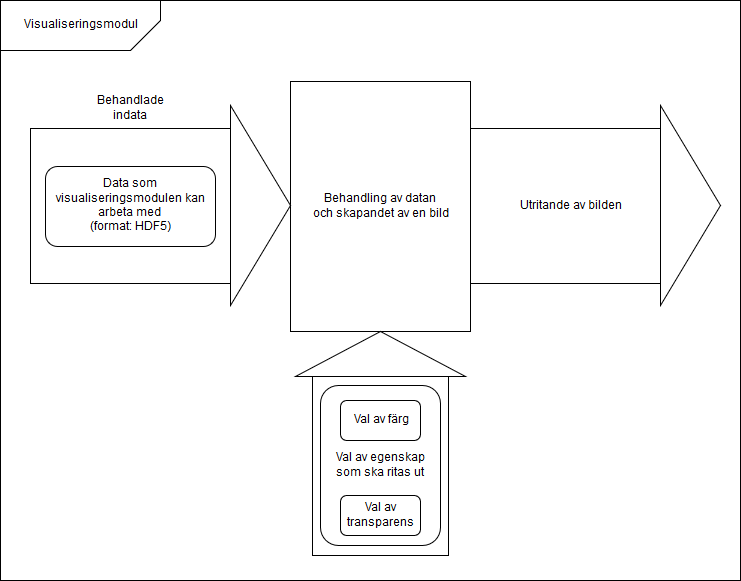
\includegraphics[scale=0.55]{Visualisering.png}
	\caption{Grov design av delsystemet Visualisering}
	\label{fig:visualisering}
\end{figure}
\subsubsection{Utriting}
Delsystemet ritar ut bilder utefter den behandlade datan. Utritningen ger en visualisering av den egenskap som modulen behandlar och kan till exempel vara en volymrendering eller en 2D-graf, beroende på vilket som är mest lättolkat. 

Utritningen görs via Inviwos inbyggda funktionalitet för att rendera via OpenGL. 

\subsubsection{Användarindata}
Användaren kan ändra inställningar som kontrollerar utseendet på visualiseringarna.
Denna indata matas in i Inviwos användargränssnitt och i inställningsrutan för en processor. Figur \ref{fig:interface} visar vad användaren ser när ser när ELF för diamant visualiseras, längst till vänster i figuren ses ett fönster mer Properties, i detta fall för processorn ELF raycasting som kan hittas i närverketlängst till höger i figuren. I mitten av bilden ligger den utritade bilden. Bilden kan roteras genom att klicka och dra i den. I Properties finns något som heter Transfer function, i den kan användaren ändra transparens/opacitet samt färg, se figur \ref{fig:transferfunction}.

\begin{figure}[H]
	\centering
	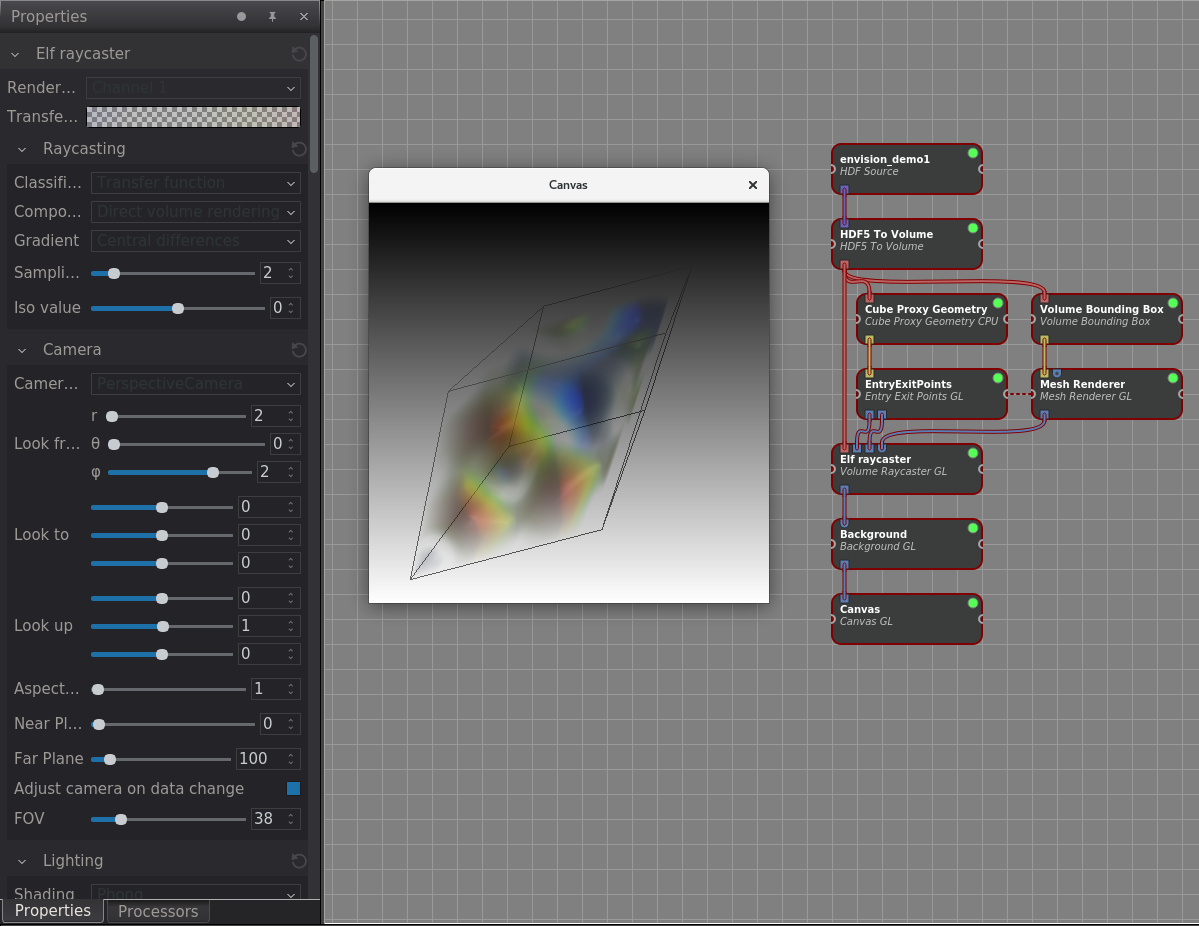
\includegraphics[scale=0.3]{inviwo_interface_elf.png}
	\caption{Bild av vad användaren ser när ELF visualiseras, i detta fall för diamant.}
	\label{fig:interface}
\end{figure}

\begin{figure}[H]
	\centering
	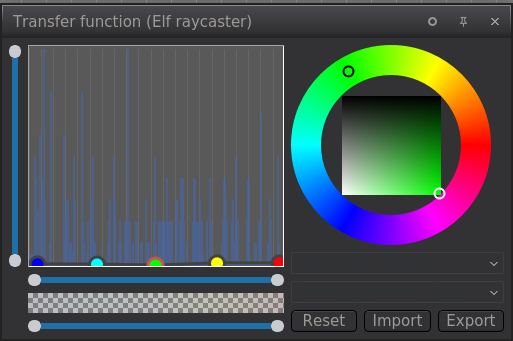
\includegraphics[scale=0.55]{transferfunction_elf.png}
	\caption{Transfer function property där transparens och färg kan ställlas in.}
	\label{fig:transferfunction}
\end{figure}

Visualiseringsfunktionaliteten läggas till i form av processorer som via Inviwo tillhandahåller inställningsmöjligheter på det sätt som beskrivits i designspecifikationen \ref{appendix:designspecifikation}. Således blir inte användarinställningar ett eget separat delsystem, utan kommer att bakas in i visualiseringssystemen. Detta görs genom att processorerna är skrivna att exponera de inställningar som användaren är menad att
justera. Inviwo kommer då automatiskt lägga till inställningarna i rutan.

\subsubsection{Interaktivitet}
Användaren kan modifiera visualiseringen genom att reglera ett intervall av värden för
någon egenskap, där full transparens fås för alla värden inom intervallet, rotera 3D-bilder etc.
Ny användarindata, som skickas in efter att den första bilden har ritats upp, skickas tillbaka till
visualiseringsmodulen för att utföra en ny rendering. 

\subsubsection{Kristallstruktur}
Kristallstruktur visualiseras som atompositioner i enhetscellen. Sfärer som representerar atomer  kan  ritas  ut  genom  volymsrendering. % figur och exempel?
I designspecifikationen, se appendix \ref{appendix:designspecifikation}, finns en mer detaljerad beskrivning av
hur detta byggs upp.
% TODO: Lägg till exempel med bild?


\subsubsection{Elektrontäthet}
Elektrontäthet visualiseras genom volymsrendering. Det är alltså sannolikheten för att hitta elektronener på olika positioner som visualiseras. %figur och exempel?
I designspecifikationen, se appendix \ref{appendix:designspecifikation}, finns en mer detaljerad beskrivning av elektrontäthet.
% TODO: Lägg till exempel med bild?

\subsubsection{ELF}
Electron Location Function (ELF) visualiseras på liknande sätt som elektrontäthet eftersom även det är volymdata som ska visualiseras. Hur ELF visualiseras beskrivs mer detaljerat i den tekniska dokumentationen, se appendix \ref{appendix:teknisk-dokumentation}.

\subsubsection{Tillståndstäthet}
Tillståndstäthet visualiseras med en 2D-graf med energn på x-axeln och tillståndstätheten på y-axeln.  %figur och exempel?.
I designspecifikationen, se appendix \ref{appendix:designspecifikation}, finns en mer detaljerad besrivning av tillståndstäthet.
% TODO: Lägg till exempel med bild?  


% TODO: Se om detta fortfarande stämmer.
\subsubsection{Fermi-ytor}
Fermi-ytor visualiseras genom att den 1:a Brillouin-zonen ritas upp för att sedan, innuti denna, rita upp en energi-isoyta (där energin är Fermi-energin). Även godtyckliga energi-isoytor kan ritas upp.  %figur och exempel?
I designspecfikationen, se appendix \ref{appendix:designspecifikation},  finns en mer detaljerad beskrivning av Fermi-ytor.
% TODO: Lägg till exempel med bild?


\section{Resultat}
\label{ch:resultat}
Projektet bestod i att skapa ett visualiseringsvektyg i Inviwo som ska kunna visualisera resultat från elektronstrukturberäkningar. Det framtagna visualiseringsverktyget ska uppfylla kraven från kravspecifikationen, nedan beskrivs några av kraven som ställts på systemet samt huruvida dessa är uppfyllda.

\subsection{Krav på systemet}
I tabell \ref{table:kravlista generella systemet} för en kravlista med några utvalda krav på det generella systemet. För samtliga krav se kravspecifikationen i appendix \ref{appendix:kravspecifikation}. Krav fem är ett krav på egenskaper som ska kunna visualiseras. Projektgruppen valde att implementera visualisering av Fermi-ytor och Total DOS, men även visualisering av ELF har implementerats. 2017 års projektgrupp i visualisering implemeterade visualisering av Total DOS och ELF, detta års arbete bestod i att uppdatera den skrivna koden för visualisering av detta till att vara kompatibel med version 0.9.9 av Inviwo. Krav 45 är ett ska krav som säger att koden ska fungera för version 0.9.9 eller senare versioner av Inviwo. Att uppdatera befintlig kod visade sig bli en stor del av arbetet eftersom tidigar versionen av Inviwo skilde sig mycket från version 0.9.9.
 
% Utkommenterade krav kanske inte är nödvändiga att ha med i kappan.

% TODO: mer beskrivningar av kraven och hur de uppfylldes?
\begin{table}[H]
\caption{Reducerad kravlista för det generella systemet.}
\begin{center}
\begin{tabular}{ |p{10mm}|p{20mm}|p{70mm}|p{15mm}|p{15mm}|}
\hline
 \textbf{Krav} & \textbf{Förändring} & \textbf{Beskrivning} & \textbf{Prioritet} & \textbf{Uppfyllt}  \\ 
\hline
 5 & Original & Systemet ska implementera, alternativt utöka befintlig implementation med, visualisering av minst två av följande egenskaper:
  \begin{itemize}
  \item Elastiska konstanter
  \item Fermi-ytor
  \item ELF (Electron Localization Function)
  \item Krafter på atomer
  \item Bandstruktur
  \item Total DOS (Density Of States)
  \item Parkorrelationsfunktionen
  \item Illustration av partiell elektrondensitet
  \end{itemize} & Ska & Ja, för Fermi-ytor, Total DOS och ELF \\
%\hline
%6 & Original & Projektgruppen ska undersöka och lära sig om samtliga egenskaper ur listan i kravet ovan. & Ska & Ja \\
\hline
7 & Original & Tillhandahållna python-moduler ska kunna anropas med enkla funktionsanrop. & Ska & Ja \\
%\hline
%8 & Original & Tillhandahållna python-moduler ska kunna hantera indata. & Ska & Ja \\
%\hline
%9 & Original & Tillhandahållna python-moduler ska kunna hantera utdata. & Ska & Ja \\
\hline
10 & Original & En beskrivning av vilka utdata en tillhandahållen python-modul producerar ska kunna erhållas. & Ska & ?? \\
\hline
11 & Original & En beskrivning av vad en tillhandahållen python-modul gör ska kunna erhållas. & Ska & Ja \\
%\hline
%12 & Original & användaren ska kunna ändra indata till python-moduler. & Ska & Ja \\
\hline
13 & Original & Användaren ska kunna välja vilken typ av visualisering som ska visas. & Ska & Ja \\
\hline
14 & Original & Användaren ska kunna länka samman olika python-moduler. & Ska & Delvis... \\
\hline
15 & Original & Systemet ska implementeras i Inviwo. & Ska & Ja \\
%\hline
%16 & Original & Tillhandahållna python-moduler ska kunna ta emot en eller flera typer av indata. & Ska & Ja \\
%\hline
%17 & Original & Tillhandahållna python-moduler ska kunna ge utdata. & Ska & Ja \\
\hline
18 & Original & Tillhandahållna python-moduler ska inte fortskrida som vanligt vid indata av fel typ. & Ska & Ja \\
\hline
19 & Original & Tillhandahållna python-moduler ska vid felaktig indata varna användaren. & Ska & Ja \\
\hline
45 & Original & Koden ska fungera för Inviwo 0.9.9 eller någon efterkommande version. & Ska & Ja \\
\hline

\end{tabular}
\label{table:kravlista generella systemet}
\end{center}
\end{table}

I listan i krav 5 valde projektgruppen att implementera visualisering av Fermi-ytor och att uppdatera befintlig kod för visualisering av total DOS. % TODO: lägg till visualiseringsbilder av dessa.
Även befintligkod för visualisering av ELF har uppdaterats, figur \ref{fig:visualisering_diamant_elf} visar visualisering av ELF-data för diamant. 
\begin{figure}[H]
	\centering
	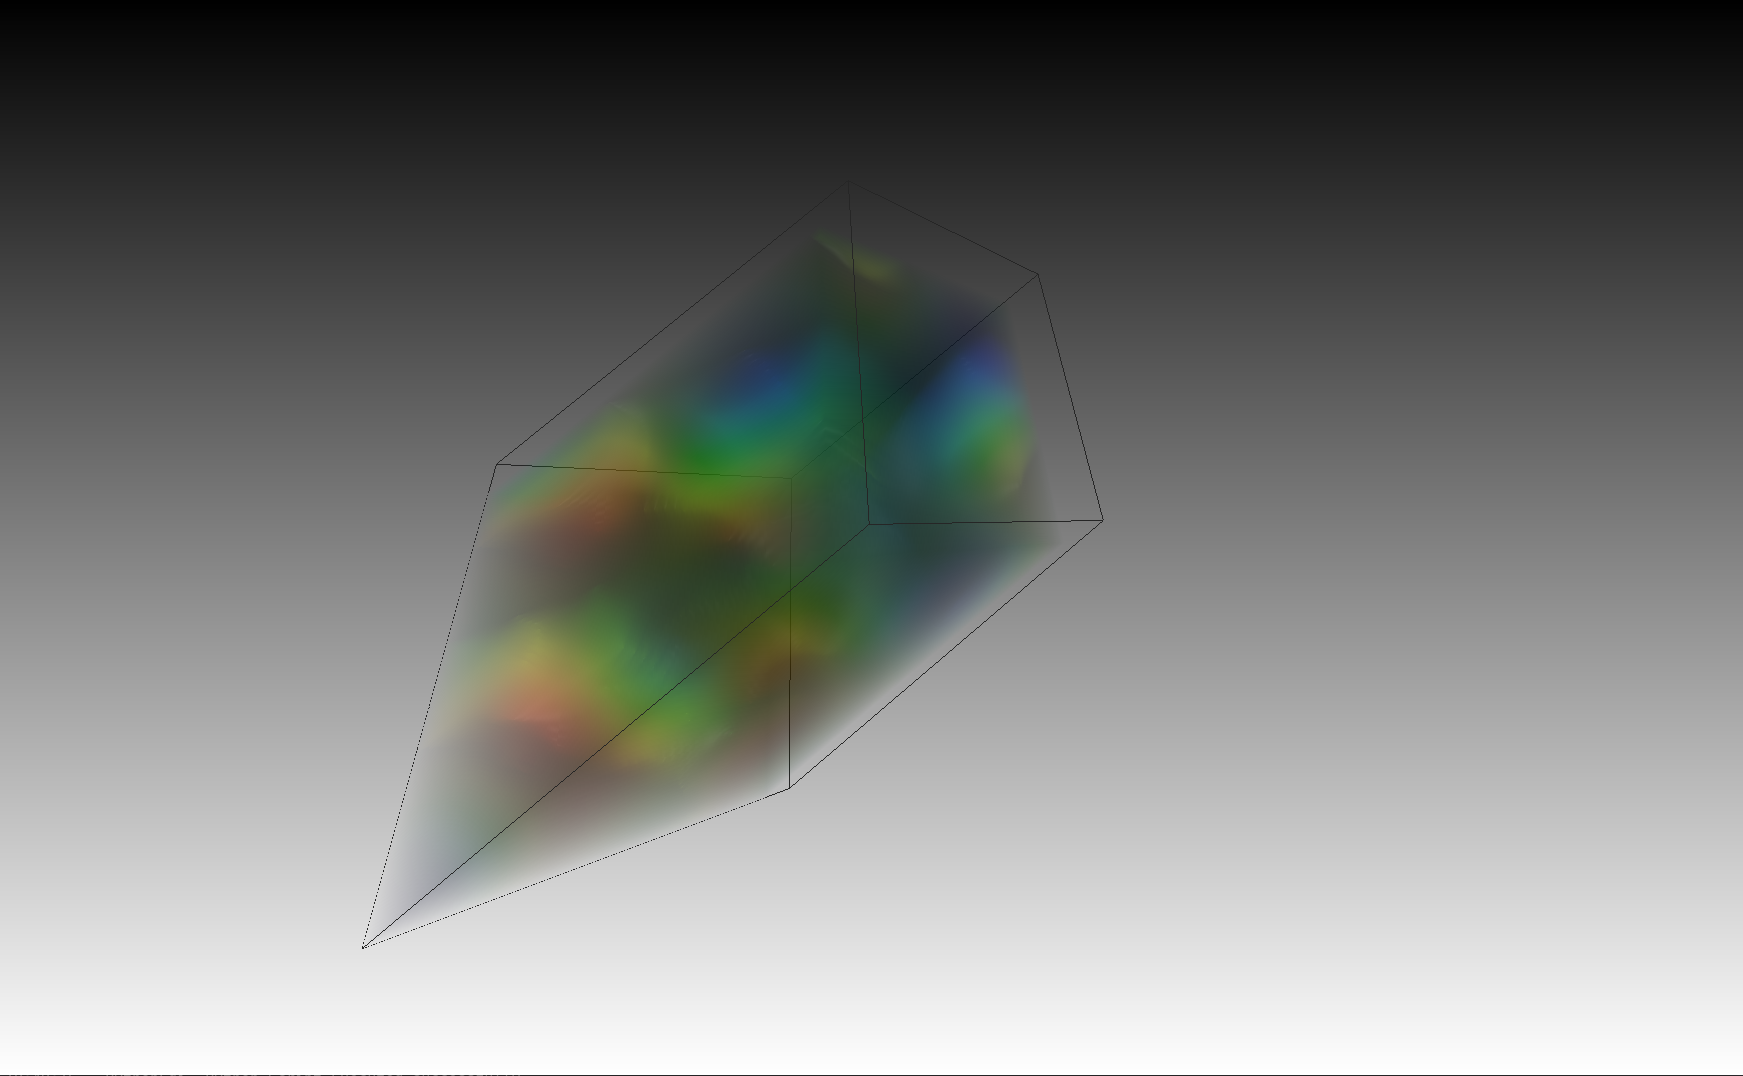
\includegraphics[scale=0.2]{Diamant_elf_visualisering.png}
	\caption{Visualisering av ELF-data för diamant.}
	\label{fig:visualisering_diamant_elf}
\end{figure}

Figur \ref{fig:visualisering_sammanlankning} visar hur visualiseringen för en sammanlänkning mellan utritande av enhetscell och utritande av ELF kan se ut, i detta fall för Al. Detta uppfyller alltså krav 14. Sammanlänkning kan göras mellan kristallstruktur och volymdata (laddningstäthet och ELF) eller mellan kristallstruktur och tillståndstäthet. Det senare gör det möjligt att se projicerad tillståndstäthet genom att klicka på enskilda atomer, vilket är krav 36 i tabell \ref{table:kravlista visualisering}.
\begin{figure}[H]
	\centering
	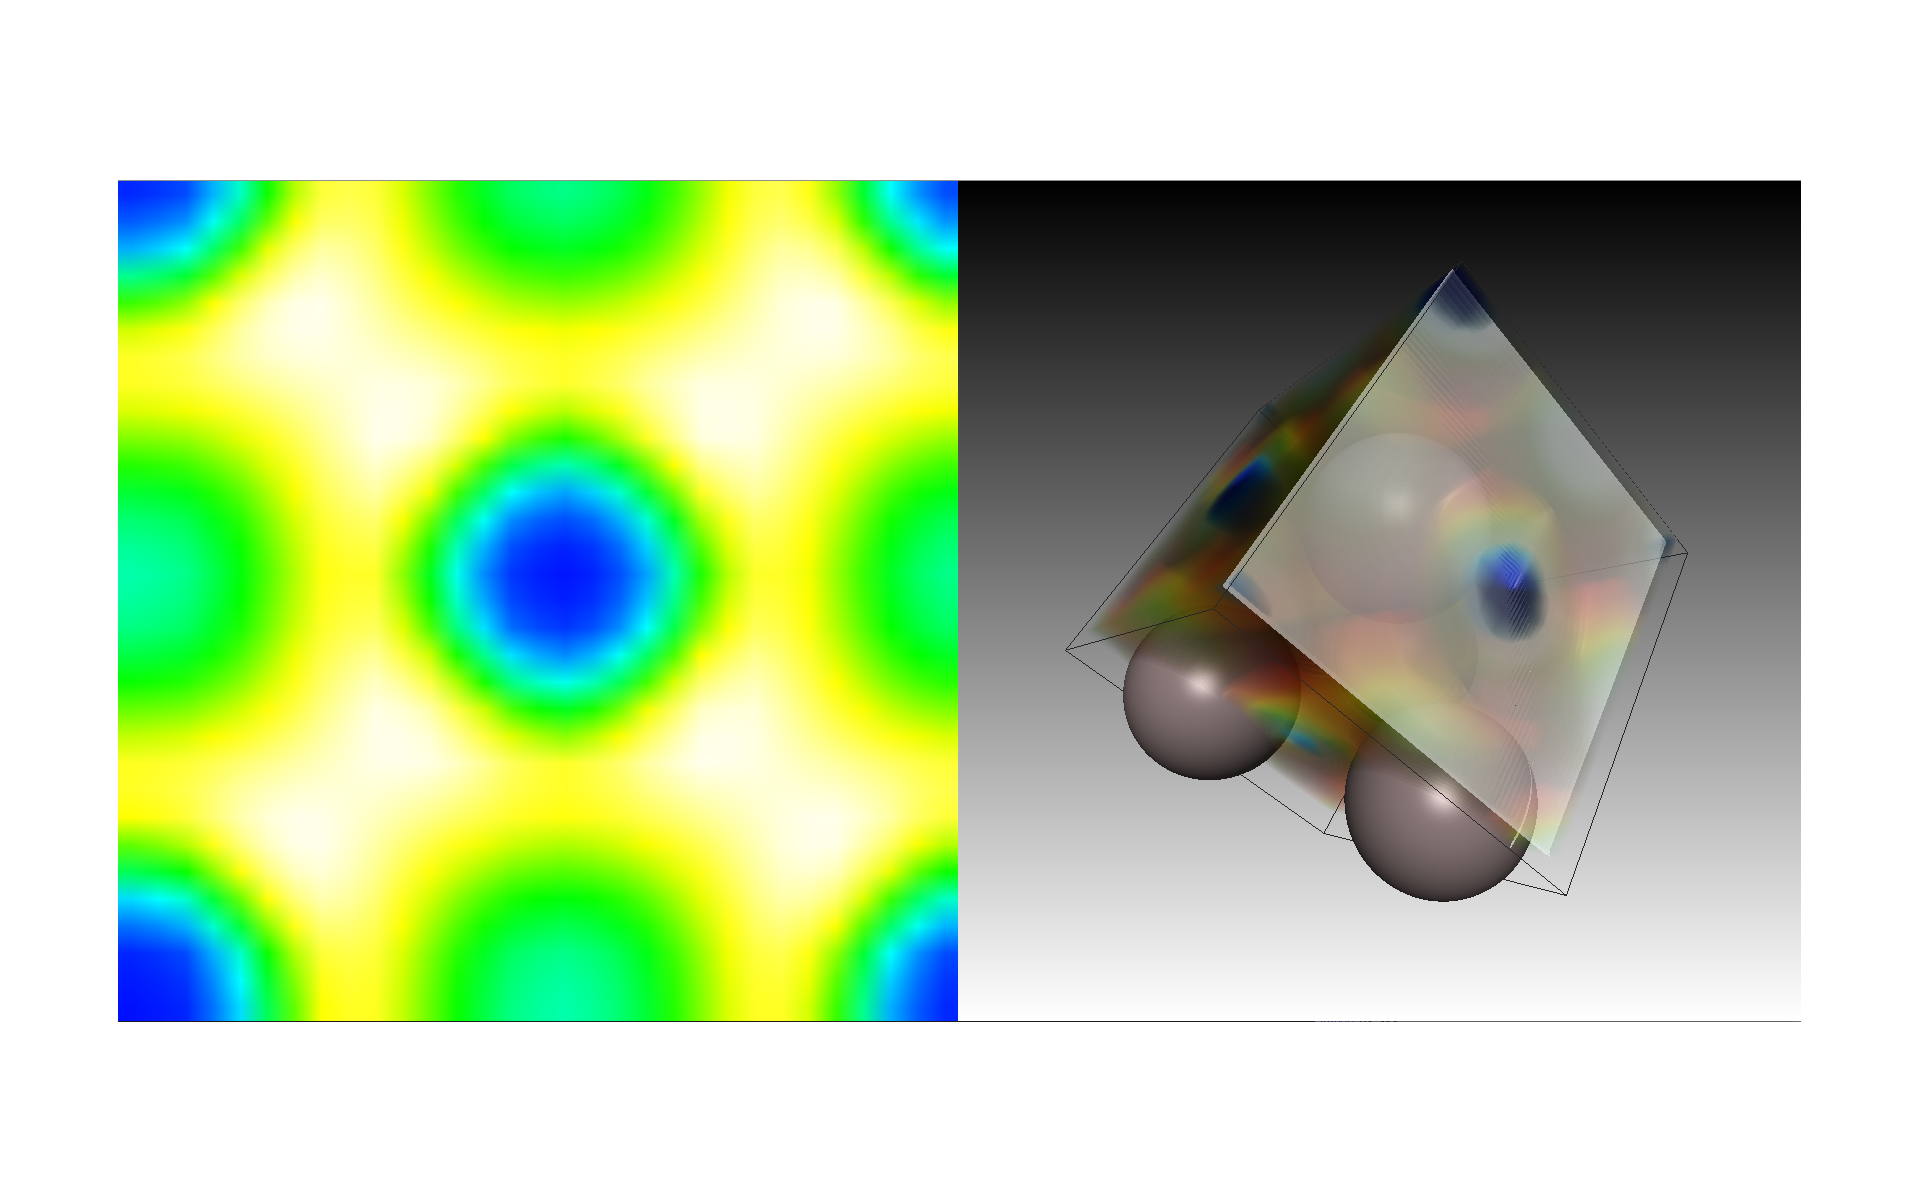
\includegraphics[scale=0.2]{sammanlankning_visualisering_Al.png}
	\caption{Data för enhetscell och ELF för Al visualiseras i samma bild.}
	\label{fig:visualisering_sammanlankning}
\end{figure}

I tabell \ref{table:kravlista datakonvertering} ses några av de krav som ställts på delsystemet för datakonvertering. Krav 24 och 29 är krav på vilket beräkningsprogram som systemet ska kunna läsa in resultat ifrån. Krav 25, 26 och 27 är krav på vilka data som ska kunna läsas in och krav 28 är ett krav på till vilket filformat som datan ska konverteras. 
\begin{table}[H]
\caption{Reducerad kravlista för delsystemet för datakonvertering.}
\begin{center}
\begin{tabular}{ |p{10mm}|p{20mm}|p{70mm}|p{15mm}|p{15mm}|}
\hline
 \textbf{Krav} & \textbf{Förändring} & \textbf{Beskrivning} & \textbf{Prioritet} & \textbf{Uppfyllt}  \\ 
\hline
24 & Original & Systemet ska kunna läsa in resultat från VASP. & Ska & Ja \\
\hline
25 & Original & Systemet ska kunna konvertera data från kristallstrukturberäkningar. & Ska & Ja \\
\hline
26 & Original & Systemet ska kunna konvertera data från elektronstrukturberäkningar. & Ska & Ja \\
\hline
27 & Original & Systemet ska kunna konvertera data från tillståndstäthetsberäkningar. & Ska & Ja \\
\hline
28 & Original & Systemet ska översätta input-filer i textformat till det binära filformatet HDF5. & Ska & Ja \\
\hline
29 & Original & Systemet bör kunna läsa in resultat från något annat beräkningsprogram, t.ex. Elk & Bör & Nej \\
\hline
\end{tabular}
\label{table:kravlista datakonvertering}
\end{center}
\end{table}


I tabell \ref{table:kravlista visualisering} ses några av de krav som ställts på delsystemet för visualisering. Visualisering av projicerad tillståndstäthet, kristllstruktur och elektrontäthet implementerades av 2017 års projektgrupp, arbetet detta år bestod i att uppdatera koden för dessa visualiseringar till att vara kompatibla för version 0.9.9 av Inviwo. 

\begin{table}[H]
\caption{Reducerad kravlista för delsystemet för visualisering.}
\begin{center}
\begin{tabular}{ |p{10mm}|p{20mm}|p{70mm}|p{15mm}|p{15mm}|}
\hline
 \textbf{Krav} & \textbf{Förändring} & \textbf{Beskrivning} & \textbf{Prioritet} & \textbf{Uppfyllt}  \\ 
\hline
36 & Original & Systemet ska visualisera projicerad tillståndstäthet härrörande till varje separat atom i en kristalls enhetscell. & Ska &  \\
\hline
37 & Original & Systemet ska viusalisera kristallstruktur som atompositioner i enhetscellen. & Ska & Ja \\
\hline
38 & Original & Systemet ska kunna visualisera den elektrontäthet som resulterar från en beräkning. & Ska & Ja \\
%\hline
%42 & Original & Systemet bör tillåta dynamisk visualisering baserad på en serie atompositioner från utdatafiler. & Bör & Nej  \\
%\hline
%43 & Original & Systemet bör tillåta att visualisering av egenskaper tillhörande atomer bara visas på vissa atomer, som kan väljas dynamiskt med ett musklick. & Bör &  \\
\hline
\end{tabular}
\label{table:kravlista visualisering}
\end{center}
\end{table}

Figur \ref{fig:visualisering_TiPO4} är ett exempel på visualisering av kristallstruktur, krav 37. Här är det TiPO4 som ritas ut där de röda sfärerna är syreatomer, de grå är titaniumatomer och de orangea är fosforatomer.
\begin{figure}[H]
	\centering
	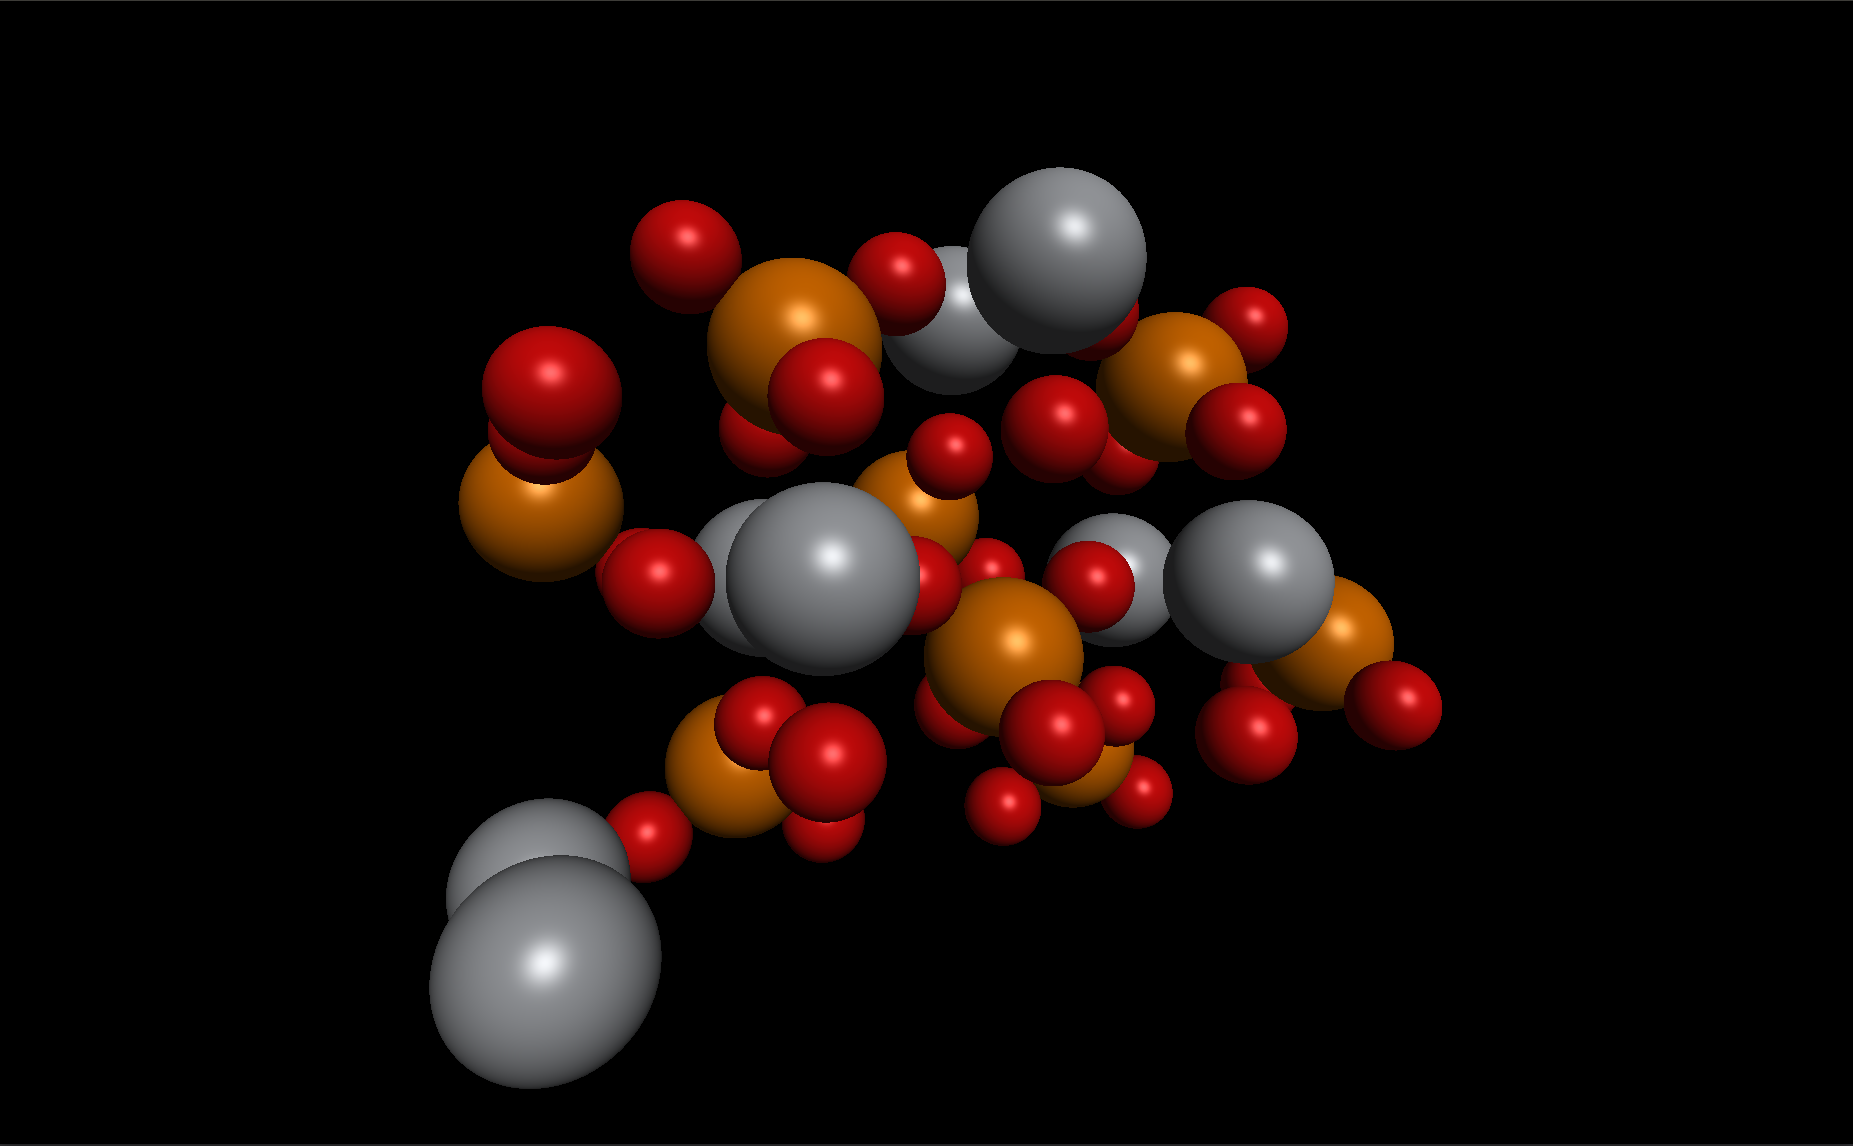
\includegraphics[scale=0.2]{TiPO4_visualisering.png}
	\caption{Visualisering av TiPO4.}
	\label{fig:visualisering_TiPO4}
\end{figure}

Figur \ref{fig:visualisering_NaCl_slice} är ett exempel på visualisering av elektrontäthet, krav 38. Här är det laddningstätheten för NaCl som ritas ut. I figur  \ref{fig:visualisering_NaCl_iso} visa också ett exempel på visualisering av laddningstäthet men i detta fall har en isoyta ritats ut för laddningstäthet lika med 0.15, även här för NaCl.

\begin{figure}[H]
	\centering
	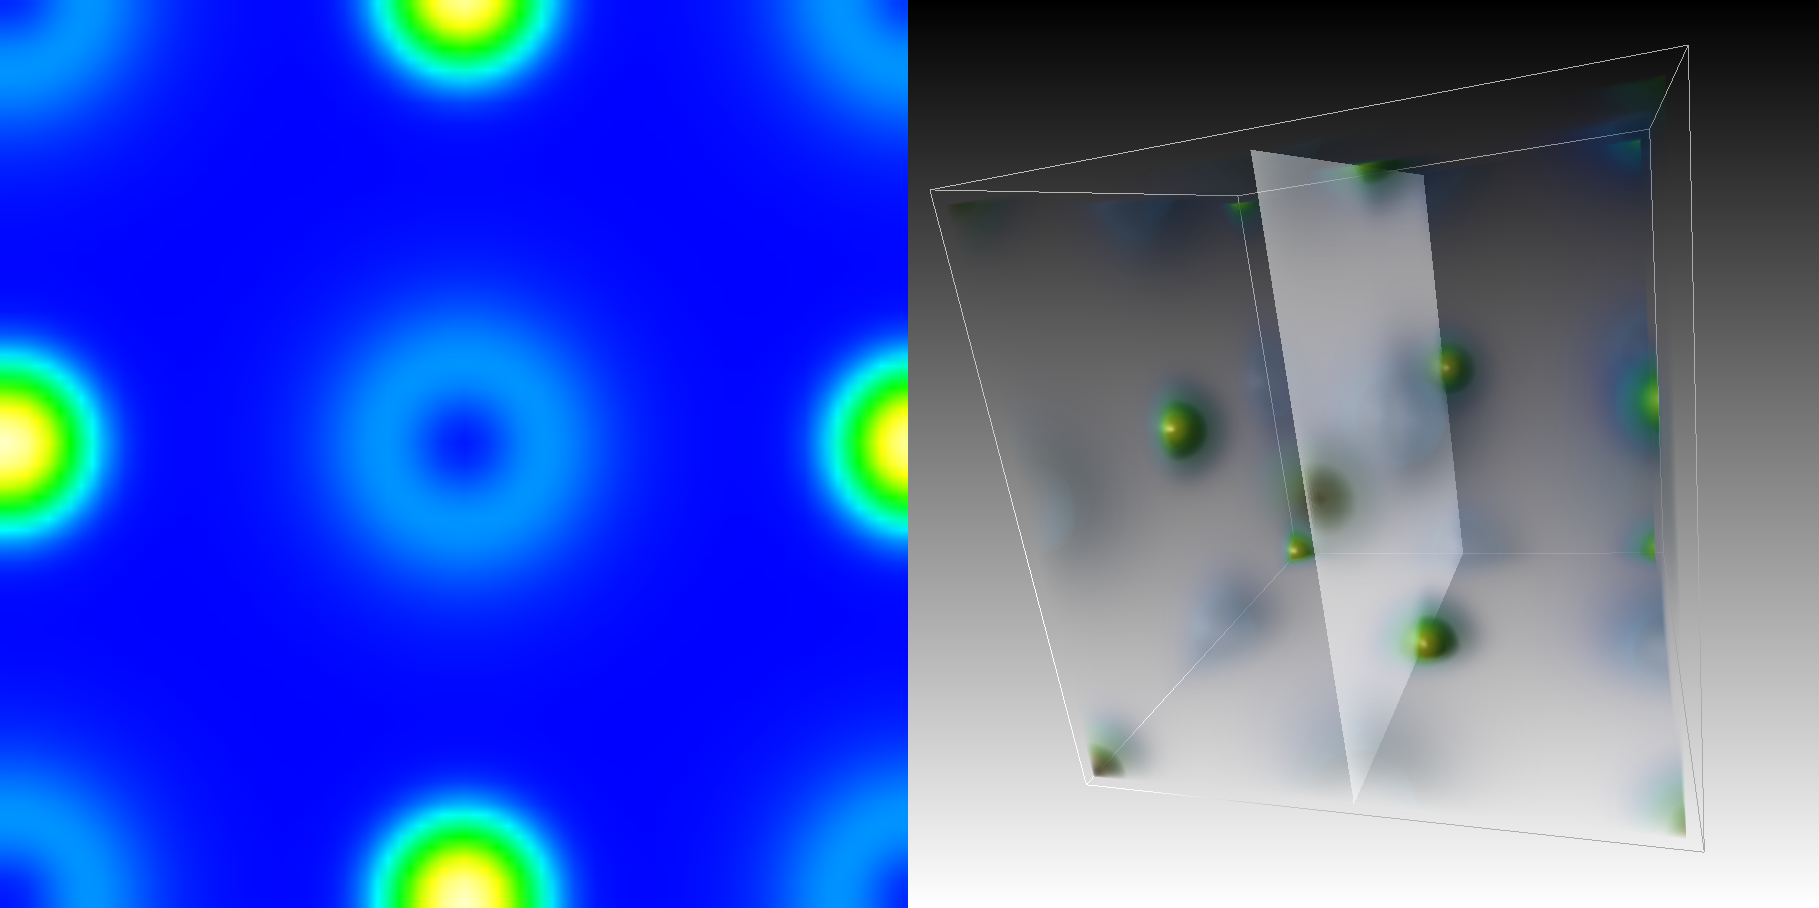
\includegraphics[scale=0.2]{NaCl_laddningstathet_slice_visualisering.png}
	\caption{Visualisering av laddningstäthet för NaCl med slice-funktion.}
	\label{fig:visualisering_NaCl_slice}
\end{figure}

\begin{figure}[H]
	\centering
	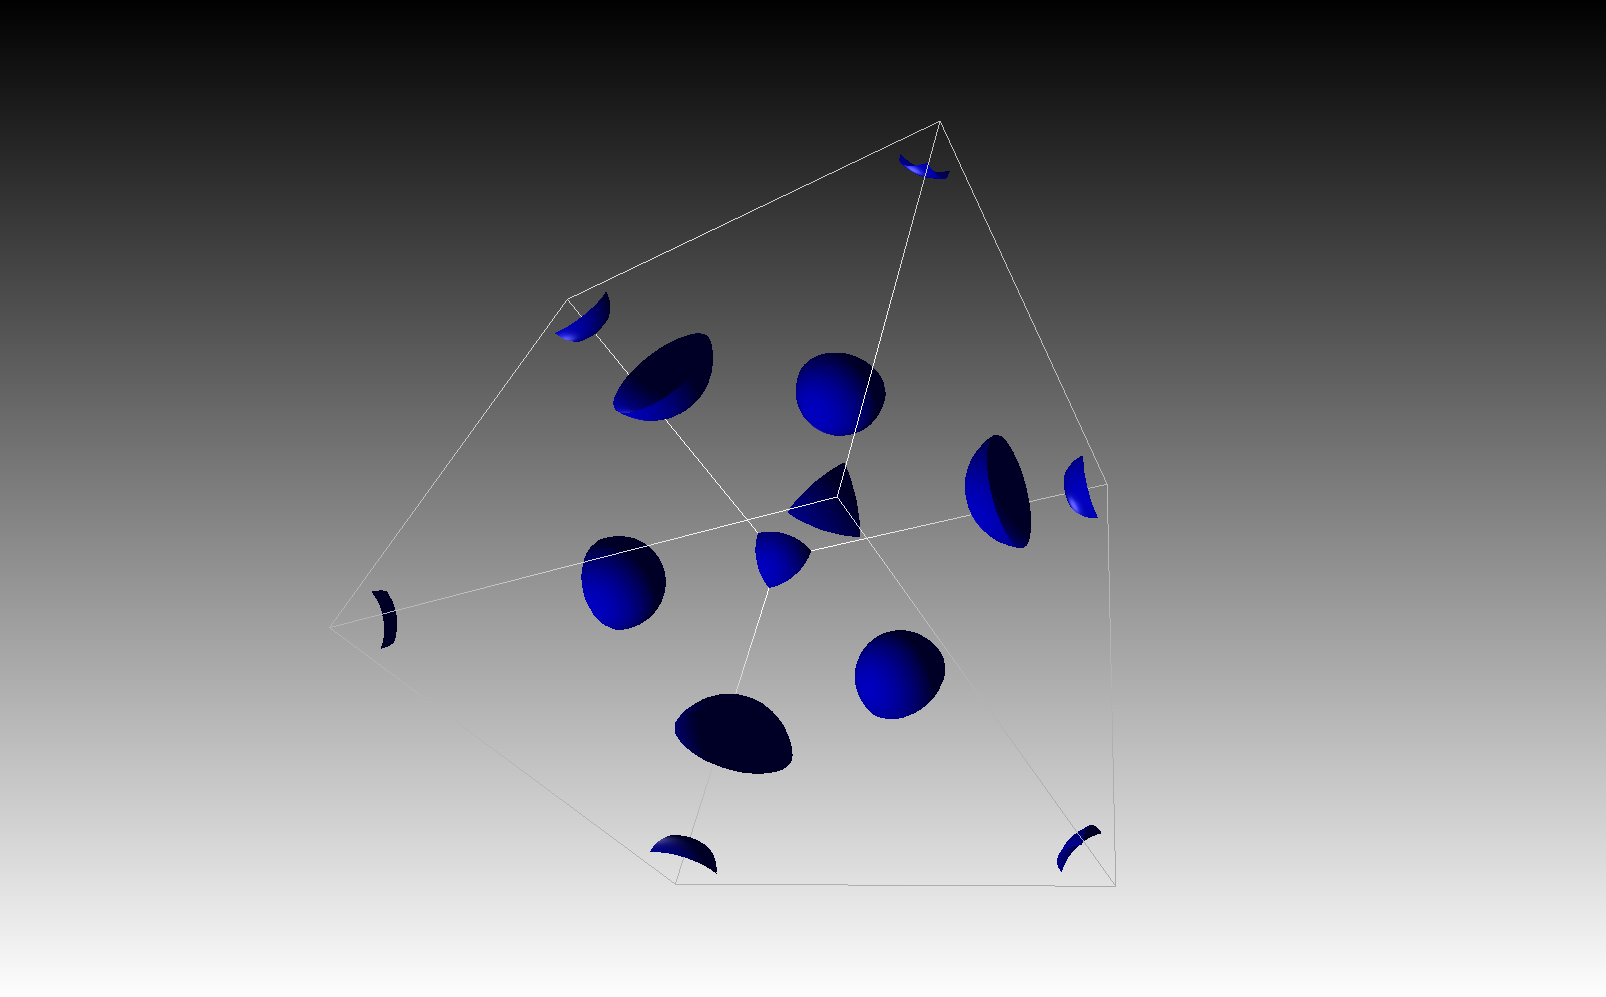
\includegraphics[scale=0.2]{NaCl_laddningstathet_iso_visualisering.png}
	\caption{Visualisering av isoyta för laddningstäthet lika med 0.15 för NaCl.}
	\label{fig:visualisering_NaCl_iso}
\end{figure}

\subsection{Användning}
För närmare beskrivning av hur verktyget används se användarmanualen i appendix \ref{appendix:användarmanual}. Det framtagna visualiseringsvertyget användas genom att öppna programmet Inviwo och där ifrån köra önskat Python-skript. Python-skript finns för samtliga typer av visualiseringar och kräver endast små ändringar i koden för att köras. Vilka ändringar som behöver göras beskrivs dels i användarmanualen men även som kommentarer i skripten. % TODO: lägg till några exempel bilder från användamanual?

% TODO: Utöka.
\section{Slutsats}
\label{ch:slutsats}
Syftet med detta projekt var inte endast att ta fram ett visualiseringsverktyg utan även att ge projektmedlemmarna erfarenhet av att arbeta i projekt. 

\subsection{Utförande}
I början av projektet bestod arbetet främst i att skriva de olika dokumenten som projektet sedan skulle utgå ifrån. Detta var dels svårt eftersom vissa delar var svåra att få grepp om utan att faktiskt sätta sig ner och göra det, och dels var det väldigt nyttigt eftersom det projektgruppen tvingades att sätta sig in i arbetet, planera och diskutera eventuella problem. 




\newpage
\addcontentsline{toc}{section}{Referenser}
\printbibliography{}

\begin{appendices}

\section{Användarmanual}
\label{appendix:användarmanual}	
	
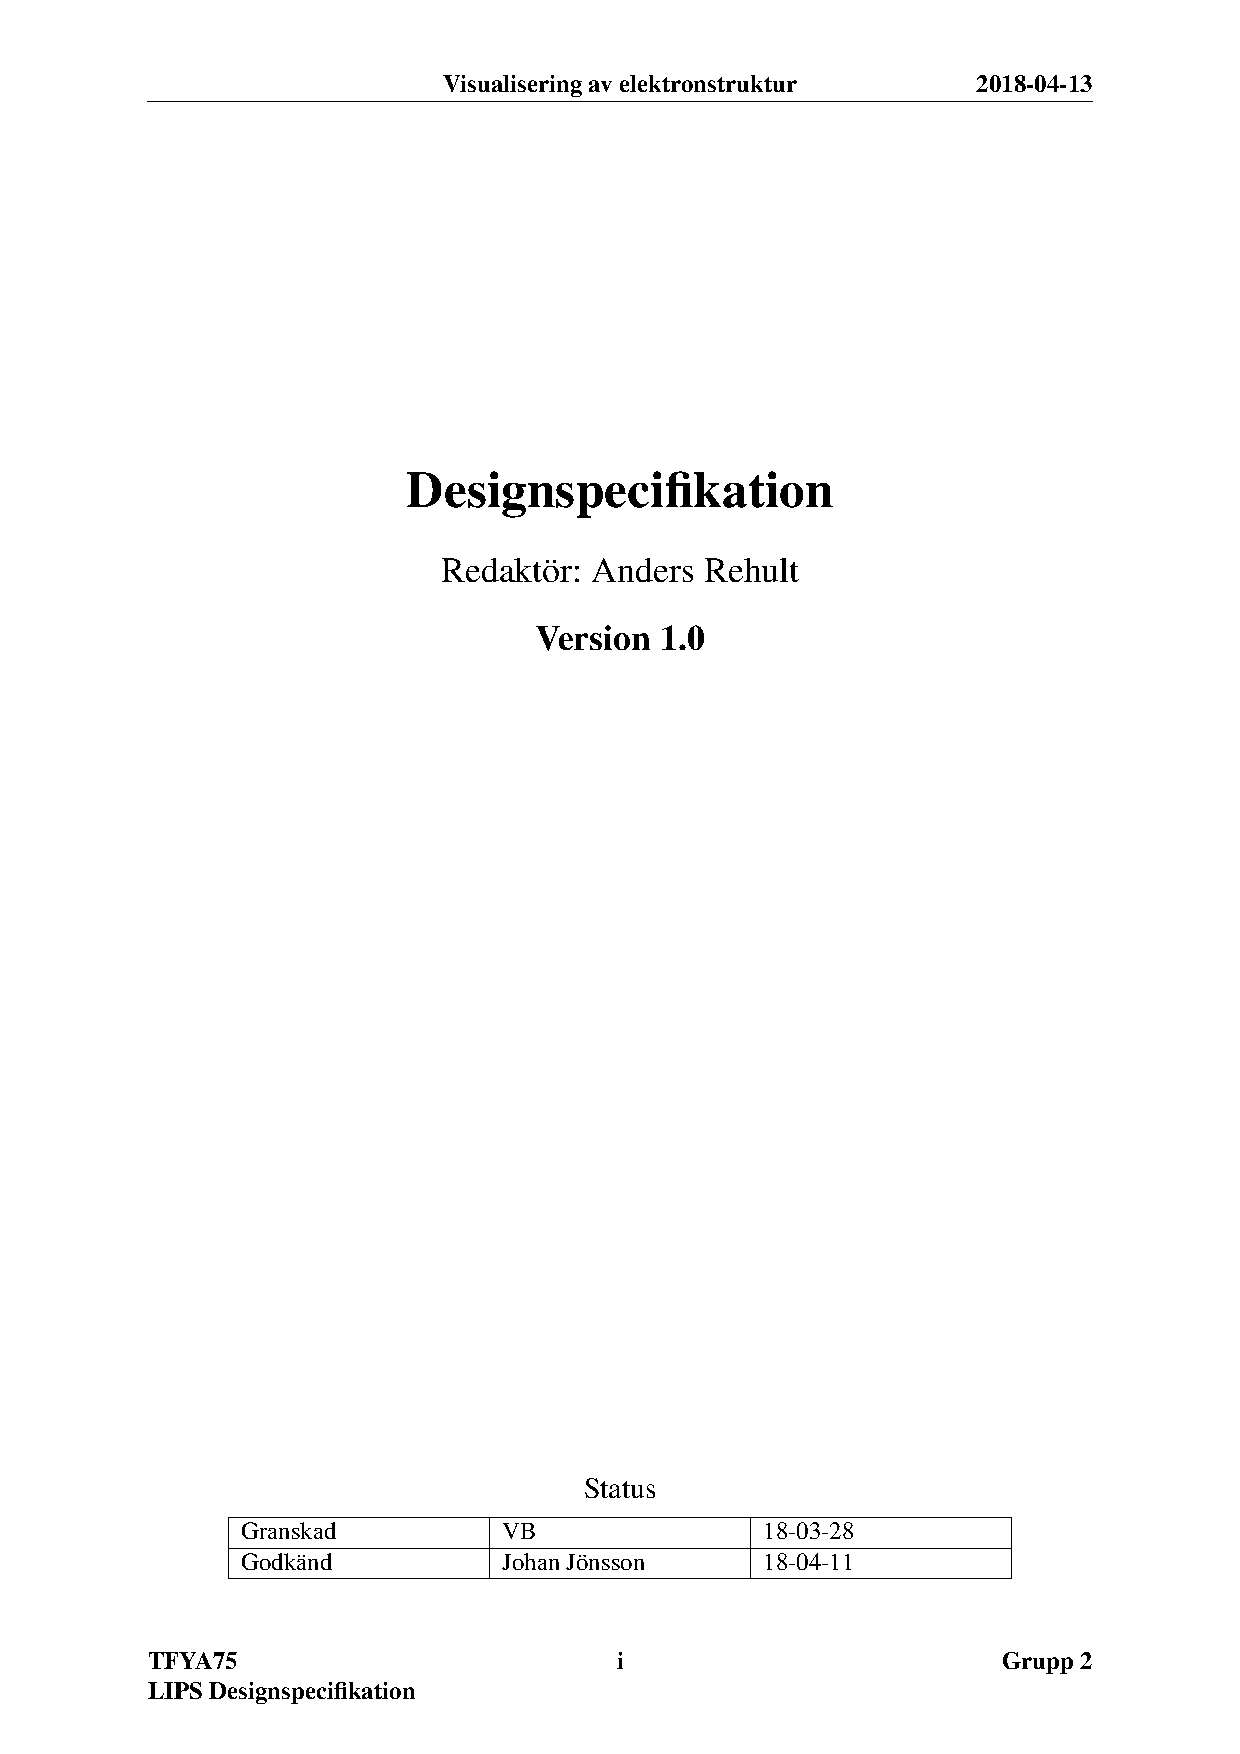
\includepdf[pages={1},pagecommand=\section{Designspecifikation}\label{appendix:designspecifikation}\thispagestyle{empty}]{designspecifikation_10.pdf} \includepdf[pages={2-}]{designspecifikation_10.pdf}
	
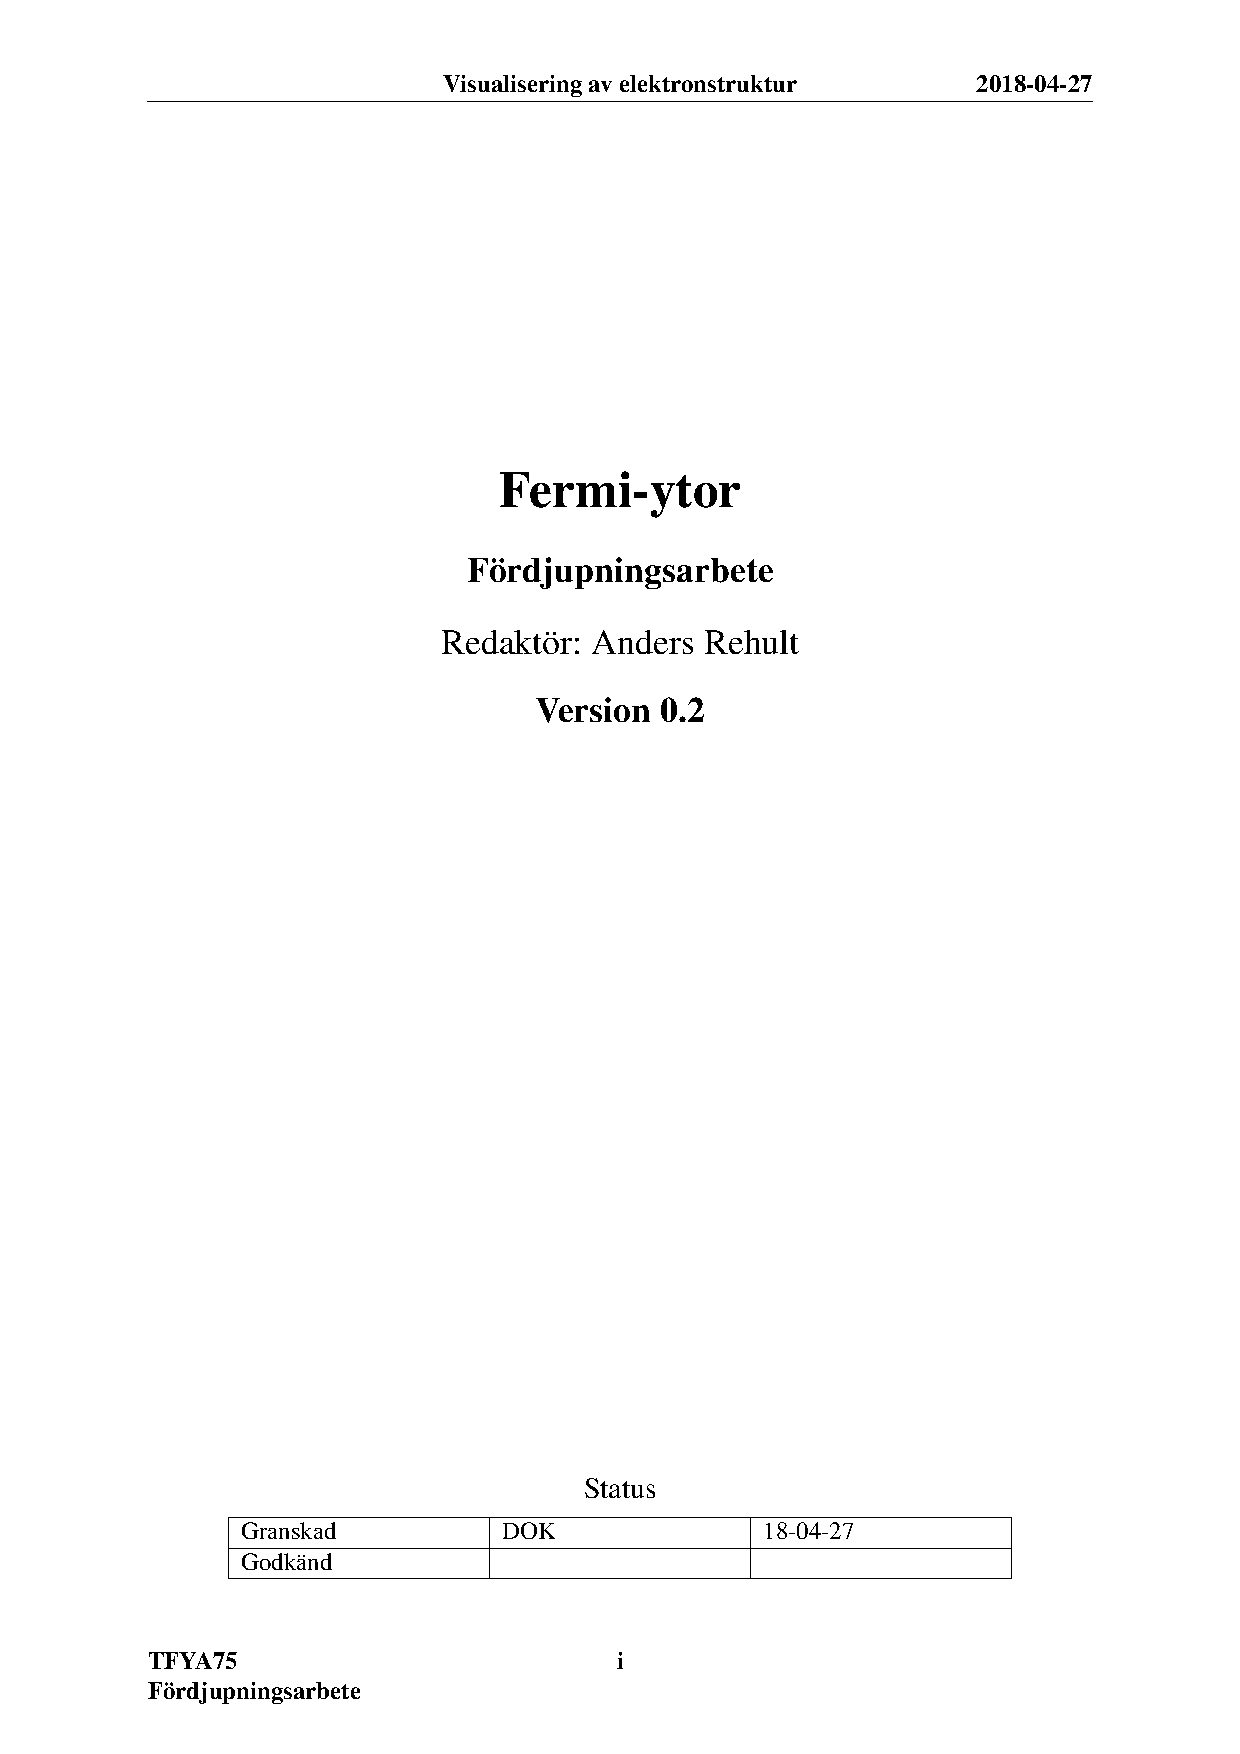
\includepdf[pages={1},pagecommand=\section{Fördjupningsarbete - Fermi-ytor }\label{appendix:fermi-ytor}\thispagestyle{empty}]{fordjupningsarbete-fermi-ytor_02.pdf}
\includepdf[pages={2-}]{fordjupningsarbete-fermi-ytor_02.pdf}

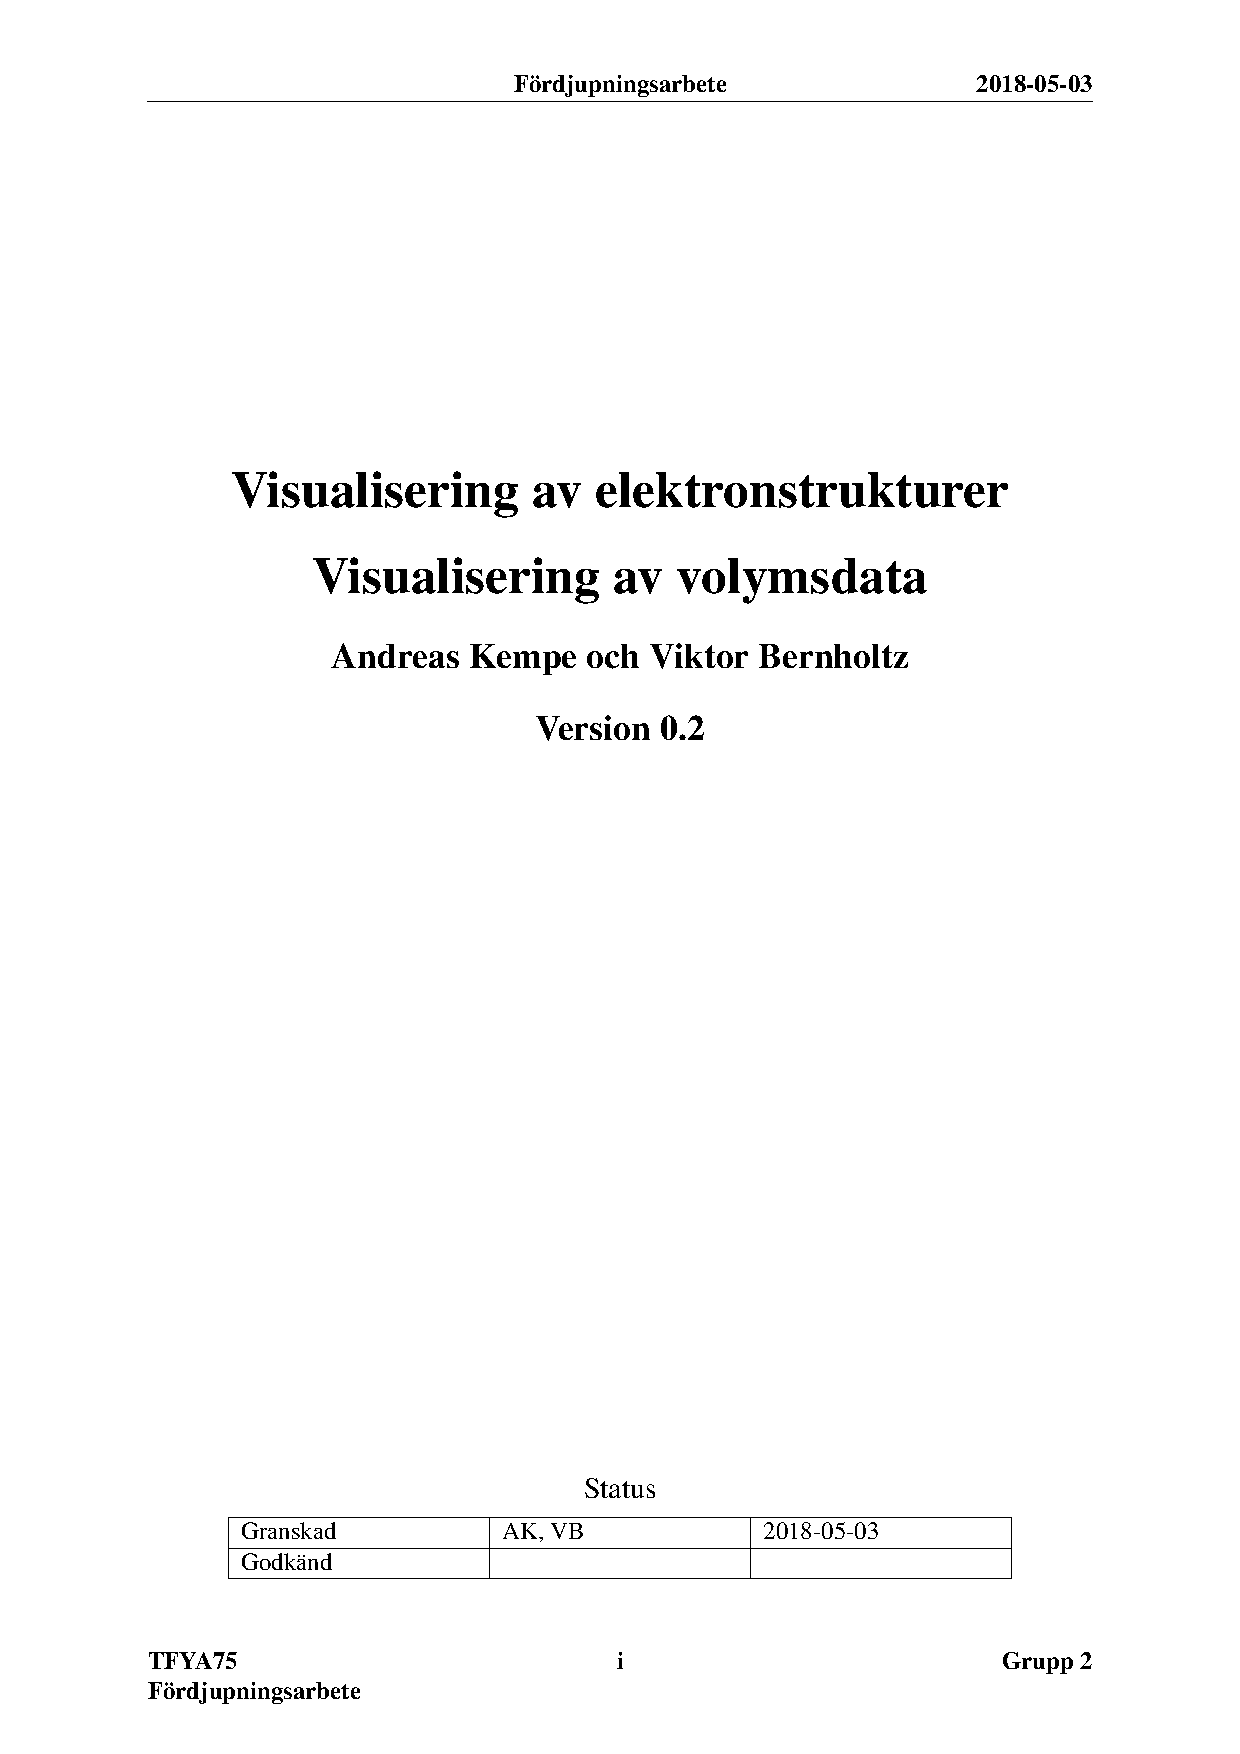
\includepdf[pages={1},pagecommand=\section{Fördjupningsarbete - Visualisering av volysmdata}\label{appendix:visualisering}\thispagestyle{empty}]{Visualisering-av-volymsdata_02.pdf}
\includepdf[pages={2-}]{Visualisering-av-volymsdata_02.pdf}
	
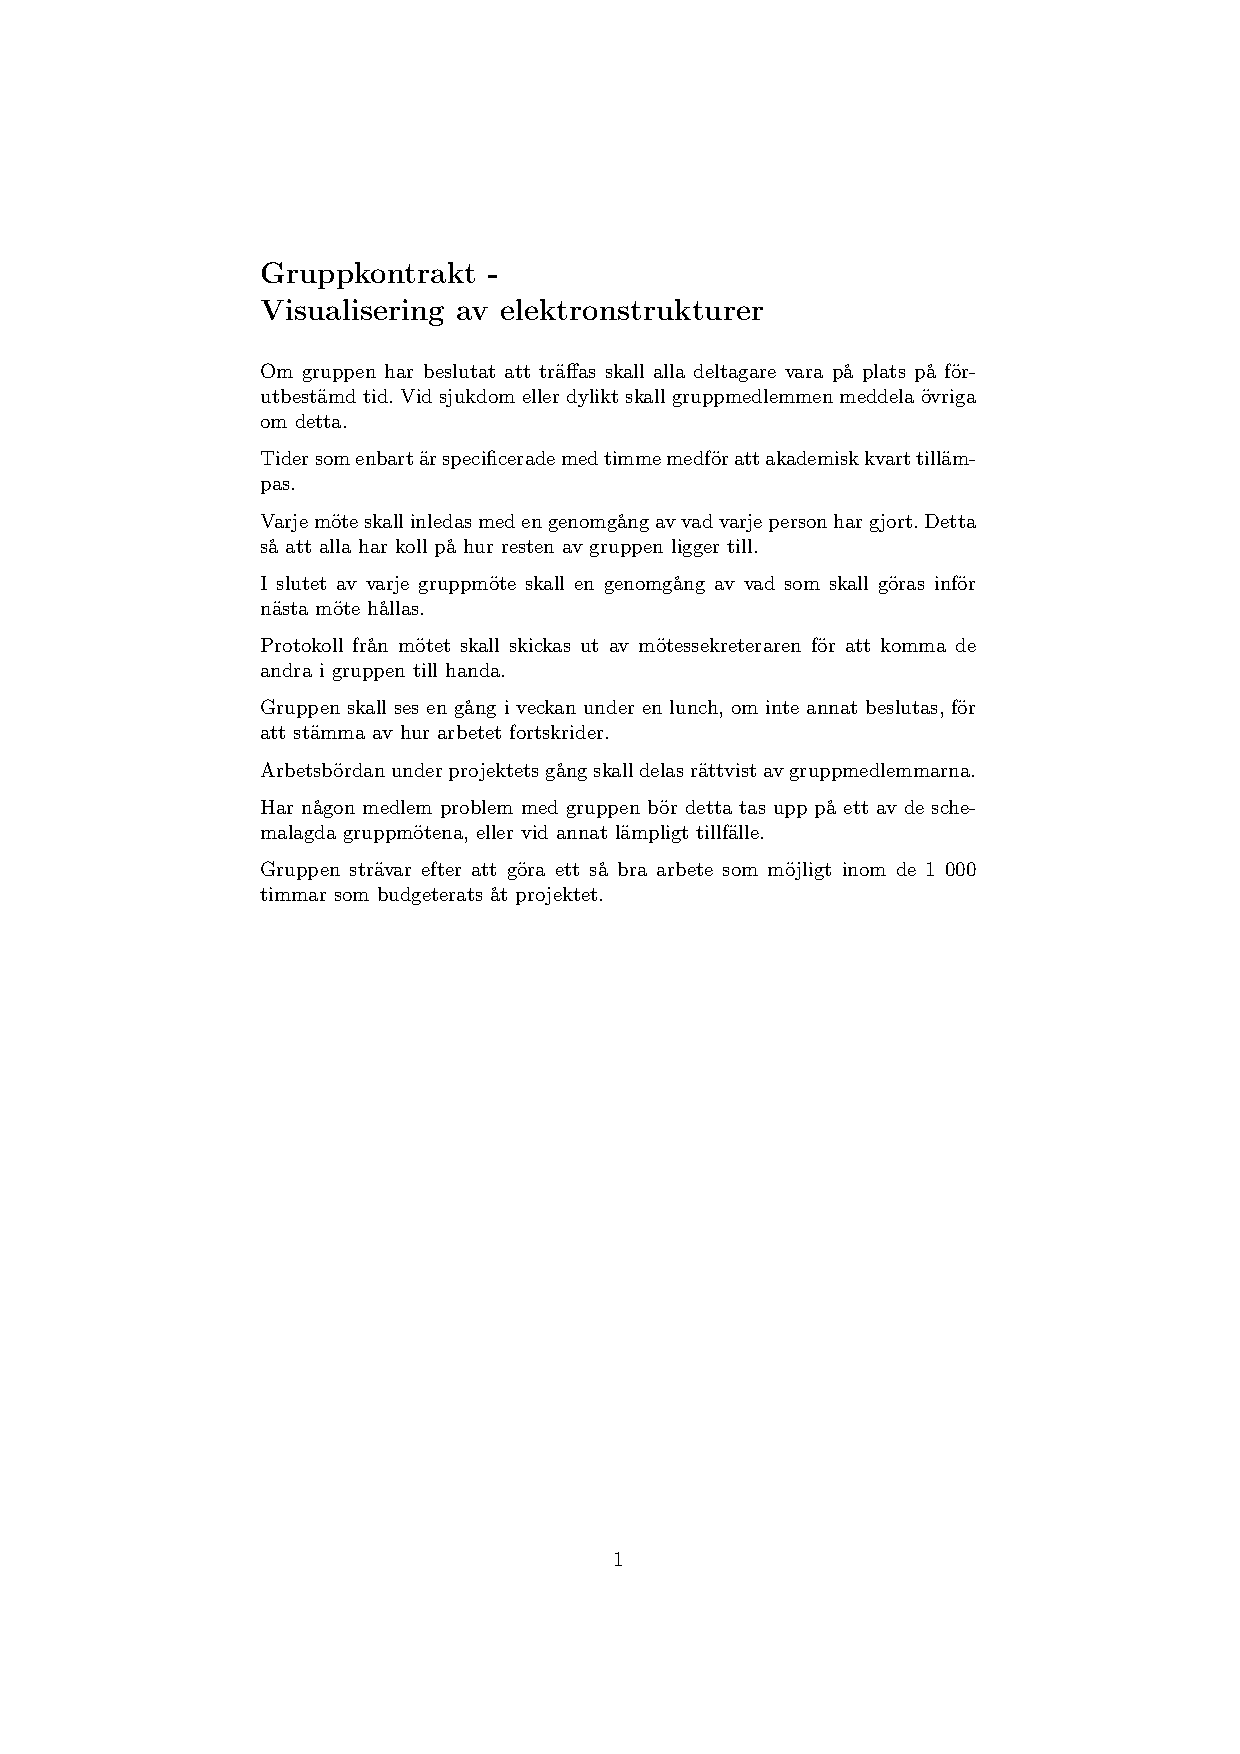
\includepdf[pages={1},pagecommand=\section{Gruppkontrakt}\label{appendix:Gruppkontrakt}\thispagestyle{empty}]{Gruppkontrakt.pdf}
	
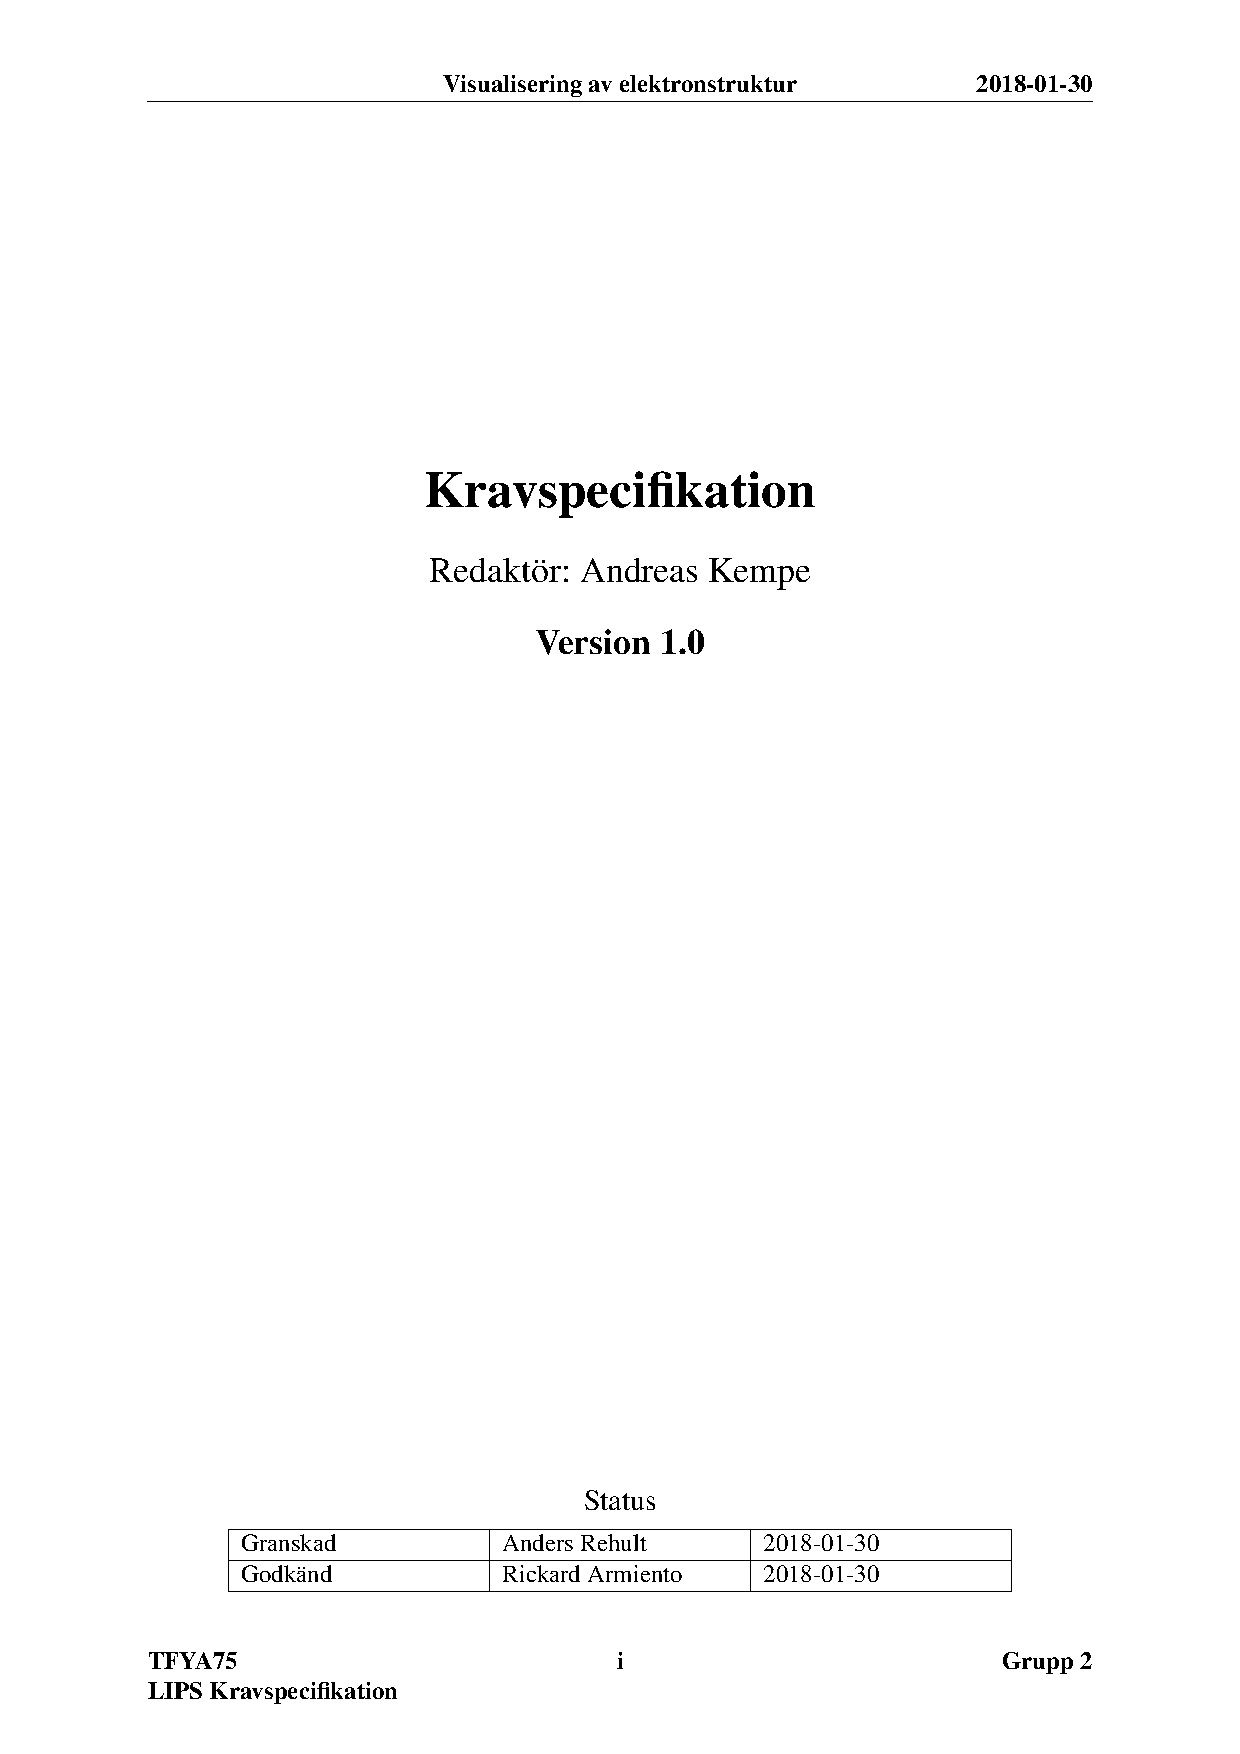
\includepdf[pages={1},pagecommand=\section{Kravspecifikation}\label{appendix:kravspecifikation}\thispagestyle{empty}]{Kravspecifikation_10.pdf}	\includepdf[pages={2-}]{Kravspecifikation_10.pdf}
	
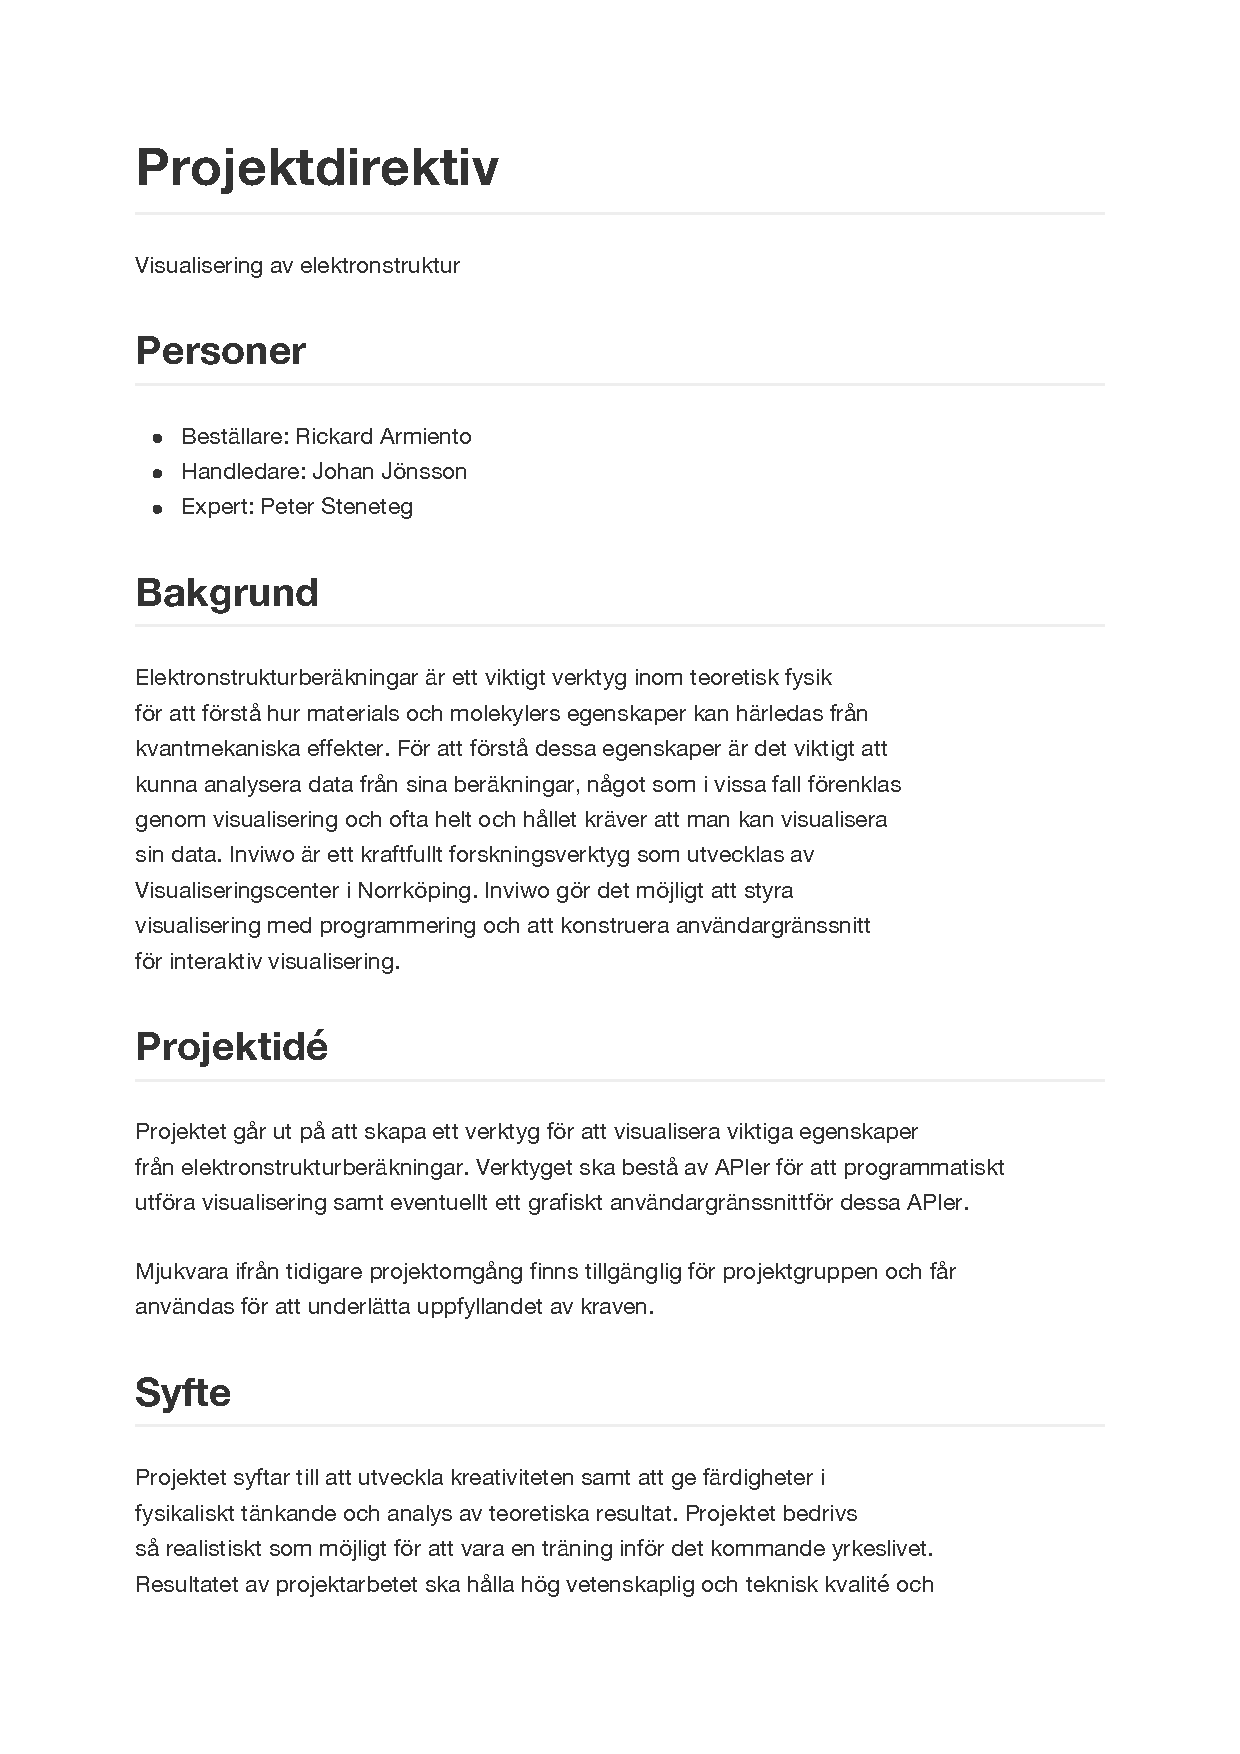
\includepdf[pages={1},pagecommand=\section{Projektdirektiv}\label{appendix:projektdirektiv}\thispagestyle{empty}]{projektdirektiv.pdf}
\includepdf[pages={2-}]{projektdirektiv.pdf}
	
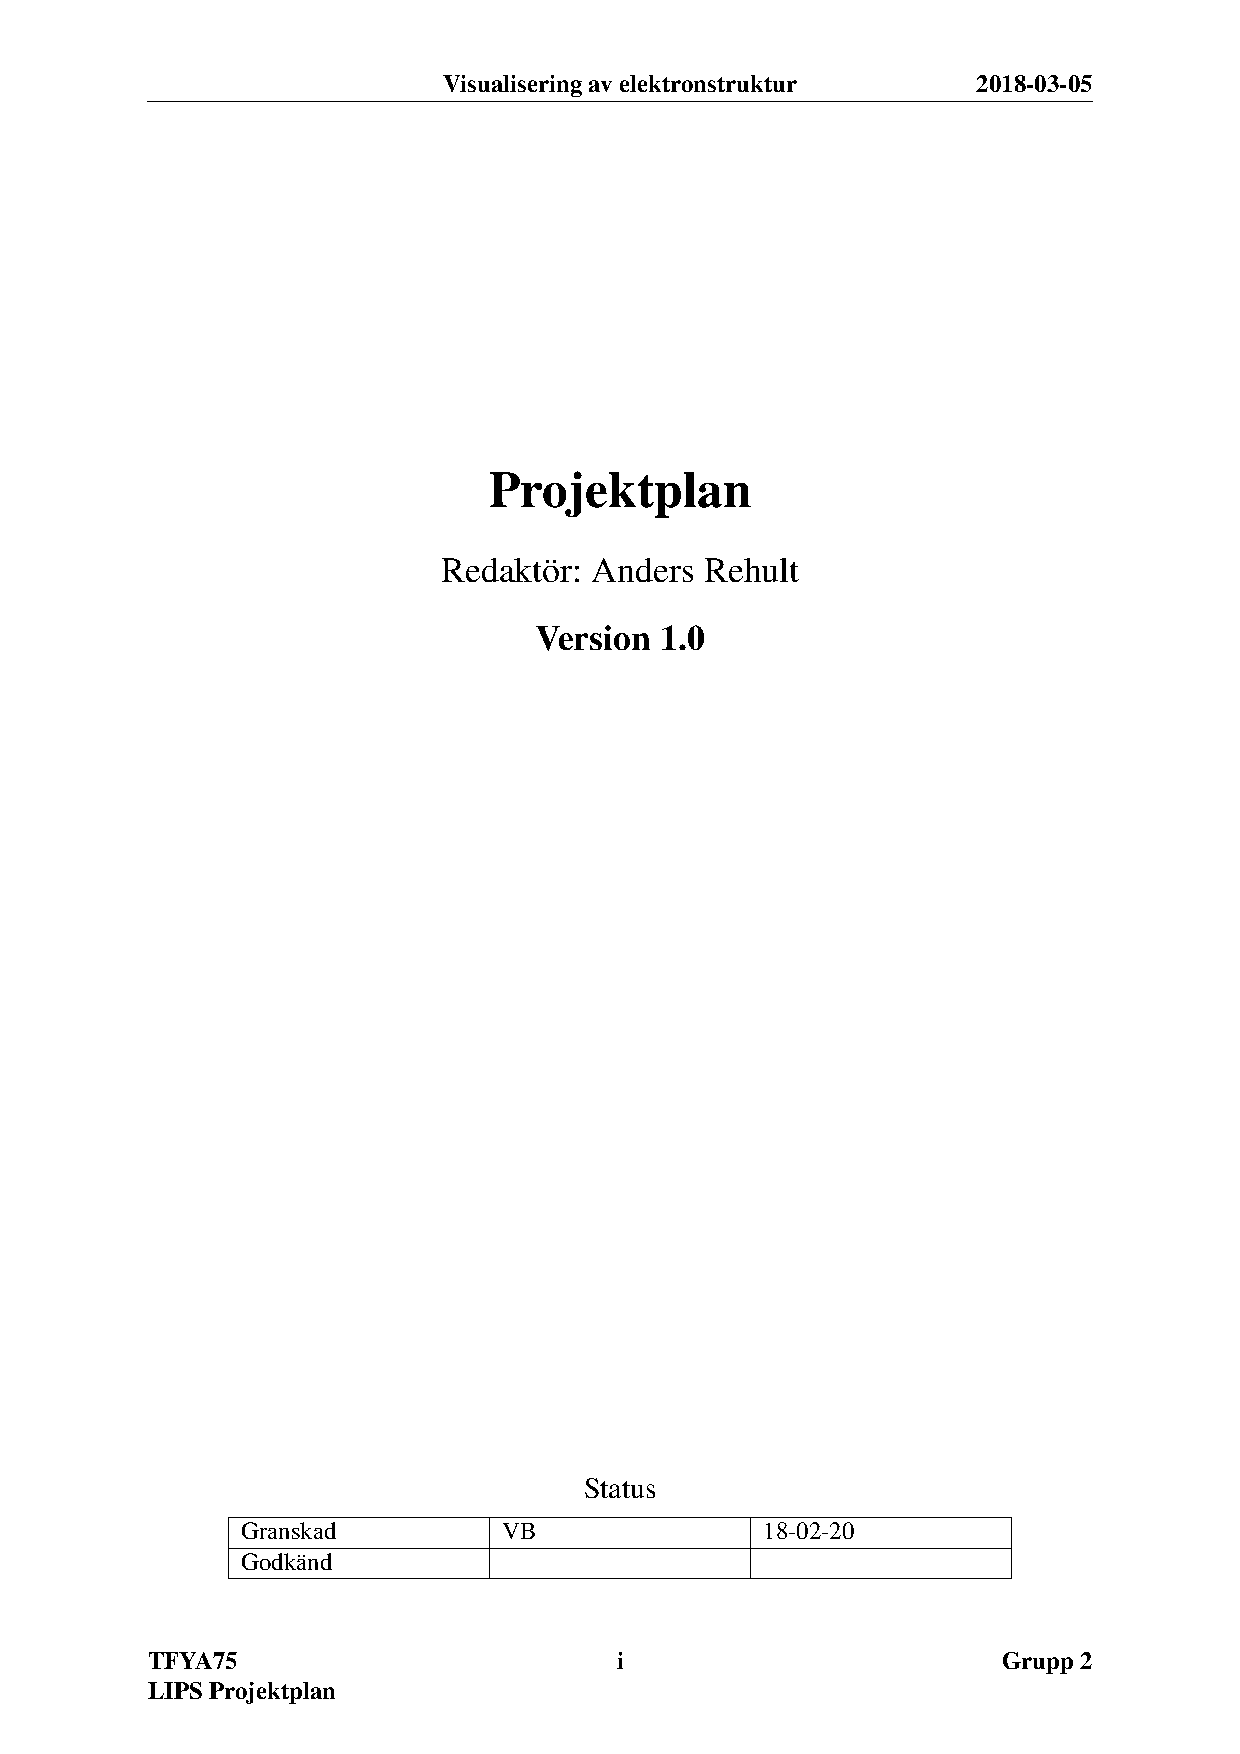
\includepdf[pages={1},pagecommand=\section{Projektplan}\label{appendix:projektplan}\thispagestyle{empty}]{projektplan_10.pdf}
\includepdf[pages={2-}]{projektplan_10.pdf}
	
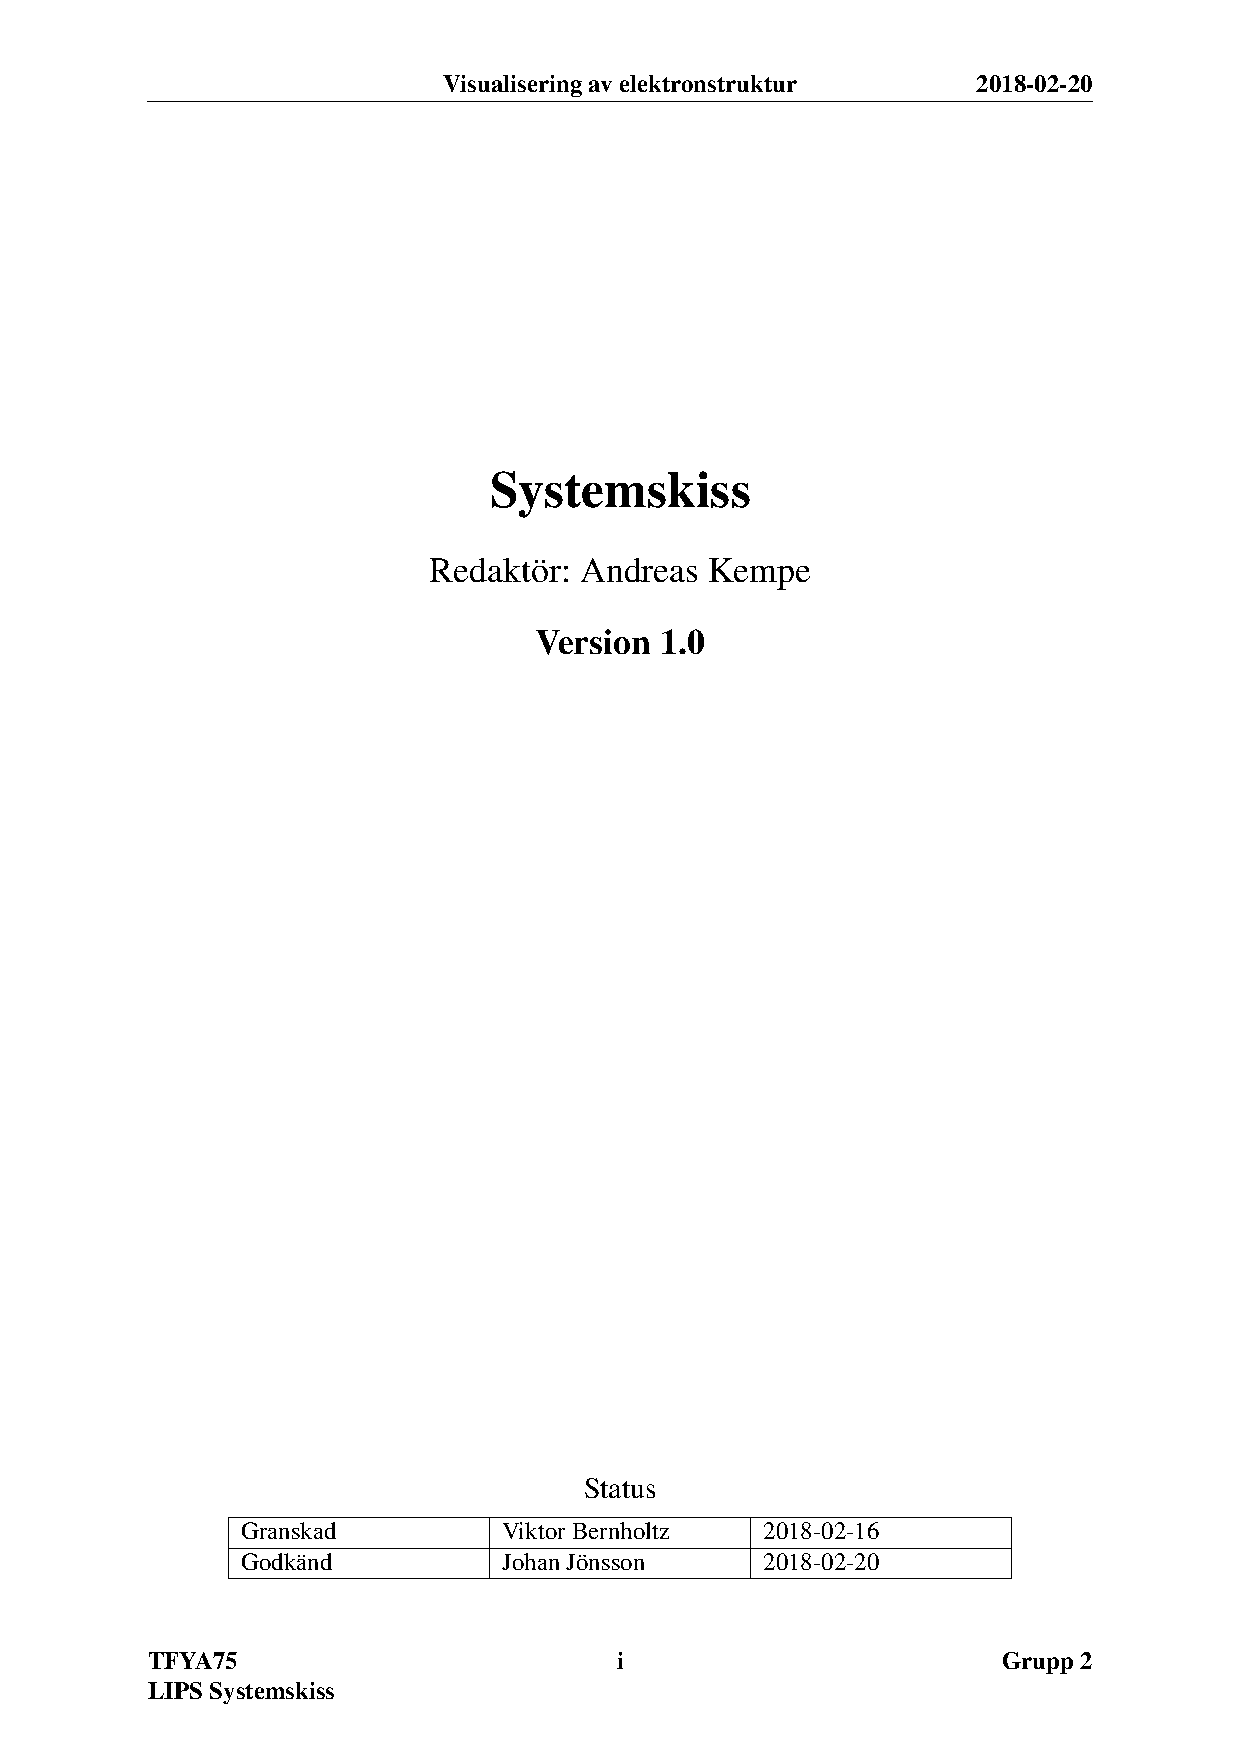
\includepdf[pages={1},pagecommand=\section{Systemskiss}\label{appendix:systemskiss}\thispagestyle{empty}]{Systemskiss_10.pdf}
\includepdf[pages={2-}]{Systemskiss_10.pdf}
	
	
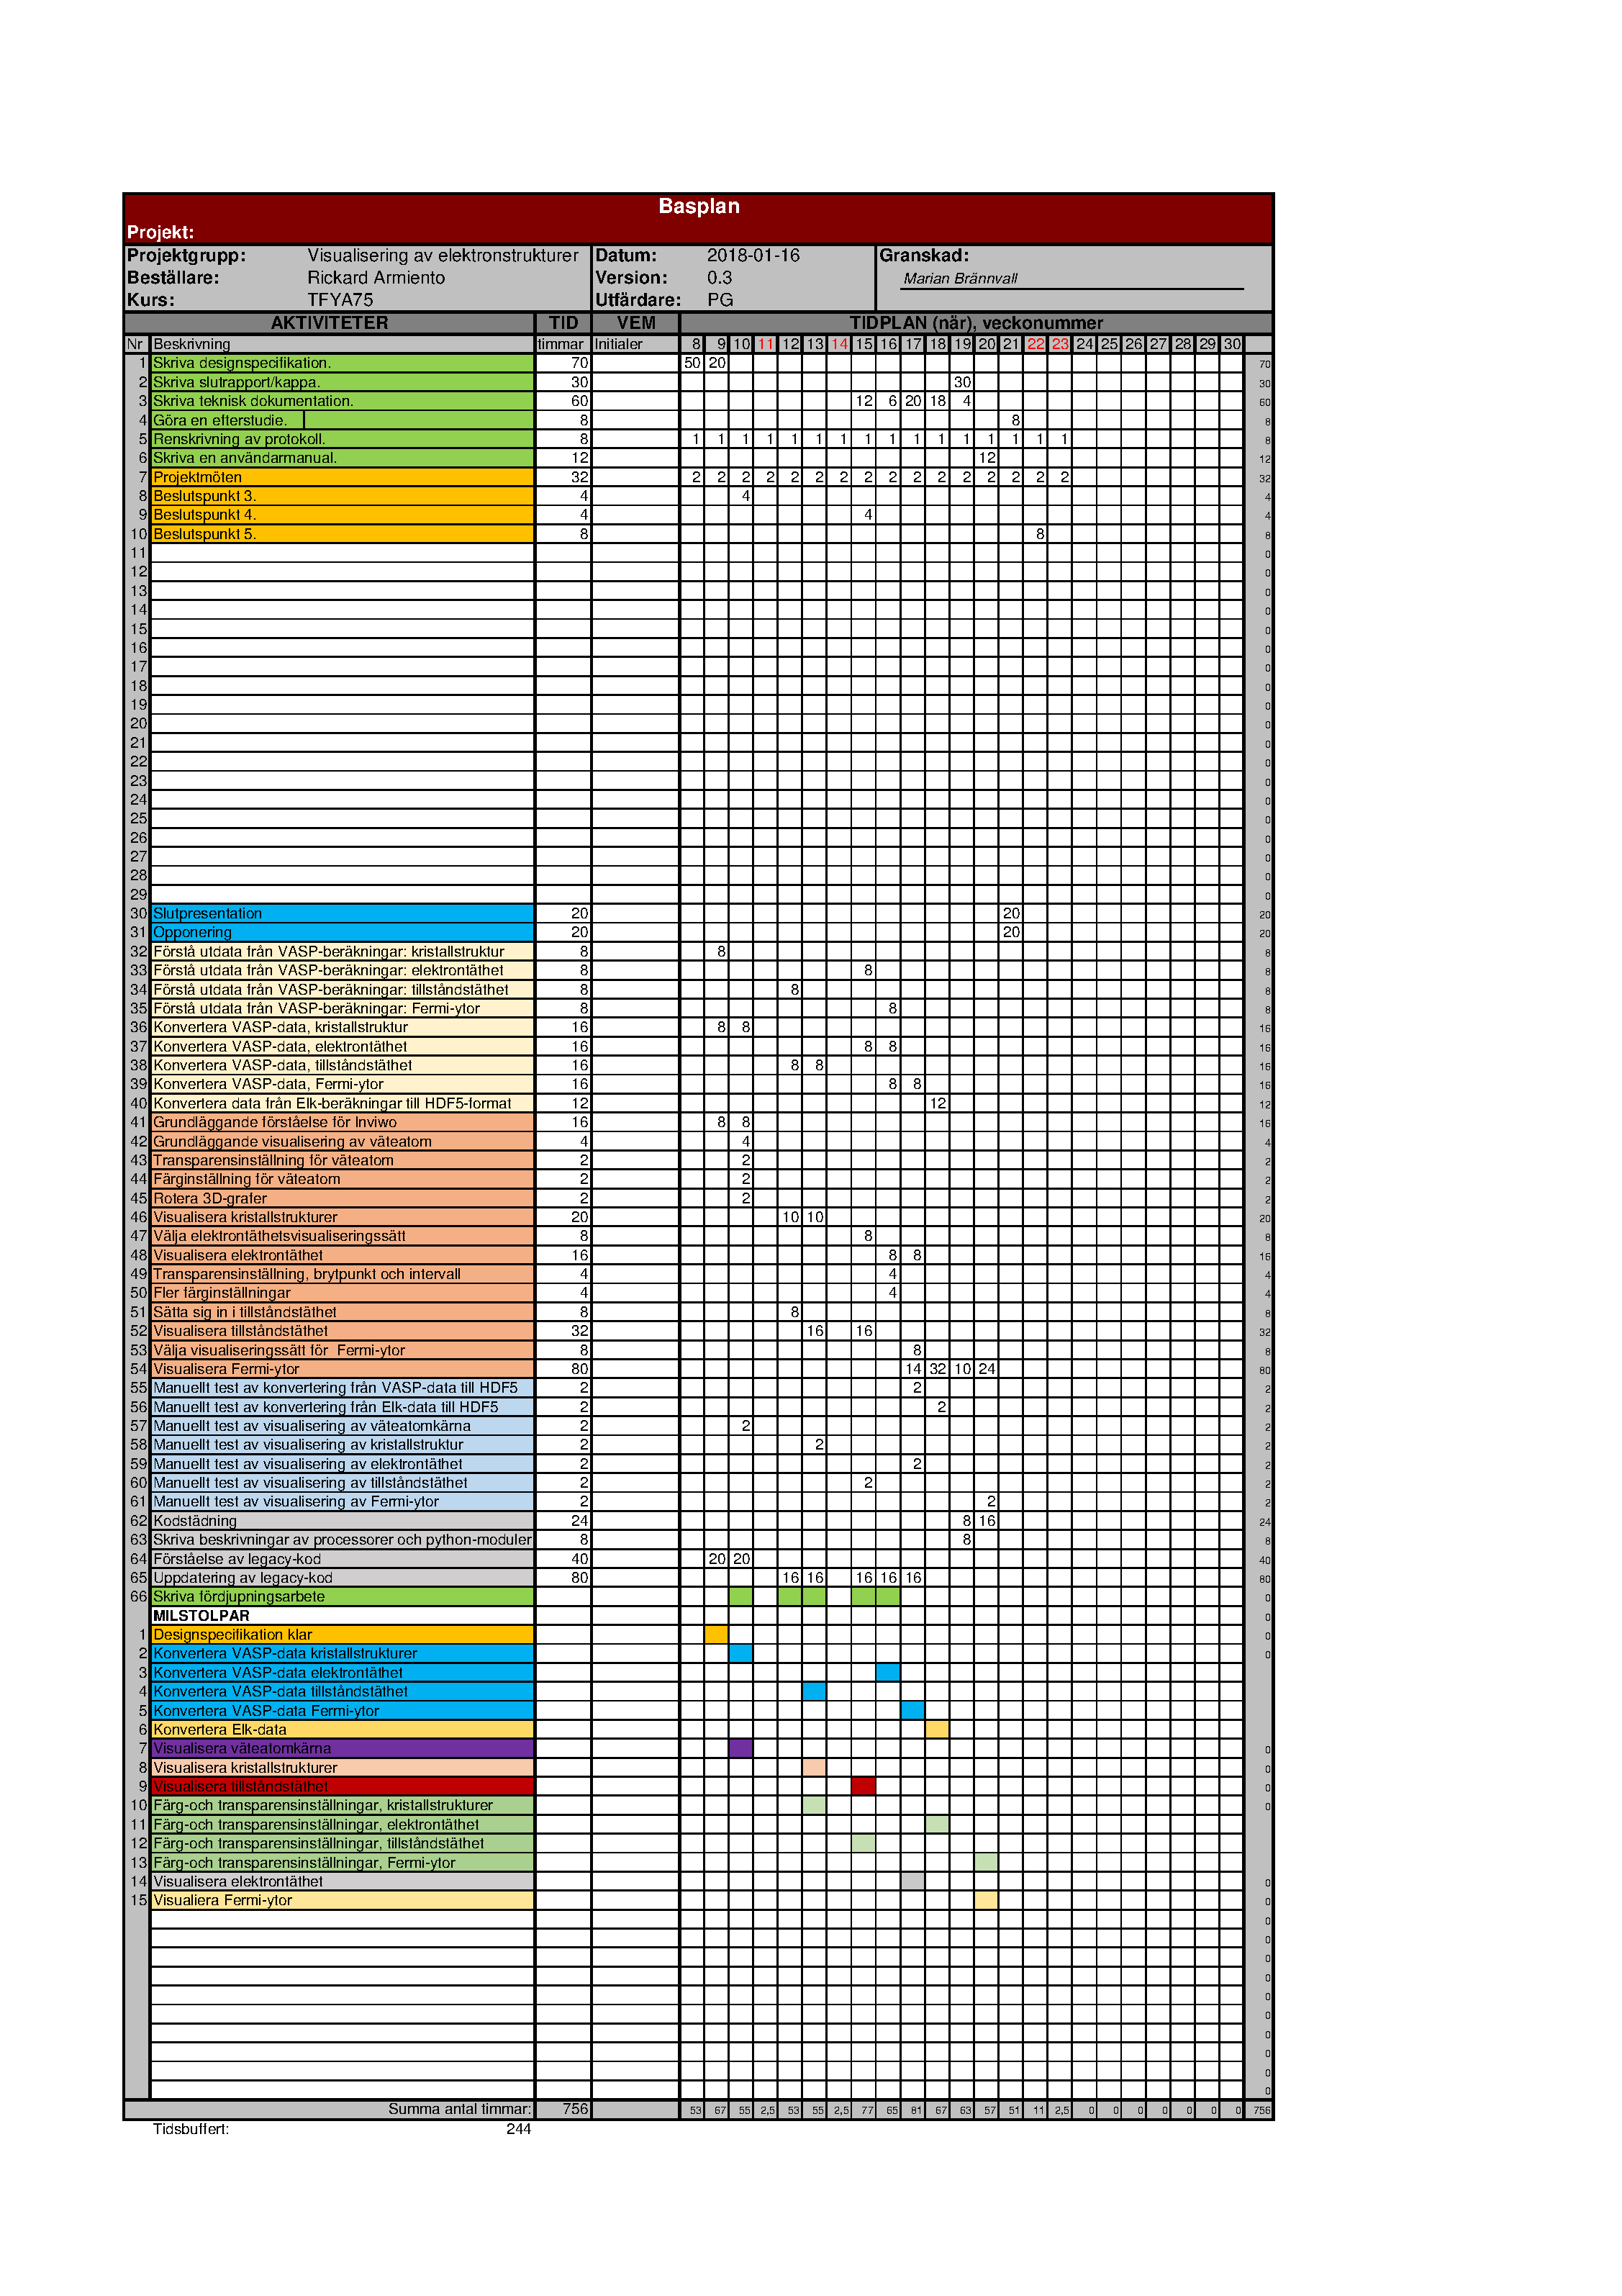
\includepdf[pages={1},pagecommand=\section{Tidplan}\label{appendix:tidplan}\thispagestyle{empty}]{tidplan_03.pdf}
	
	
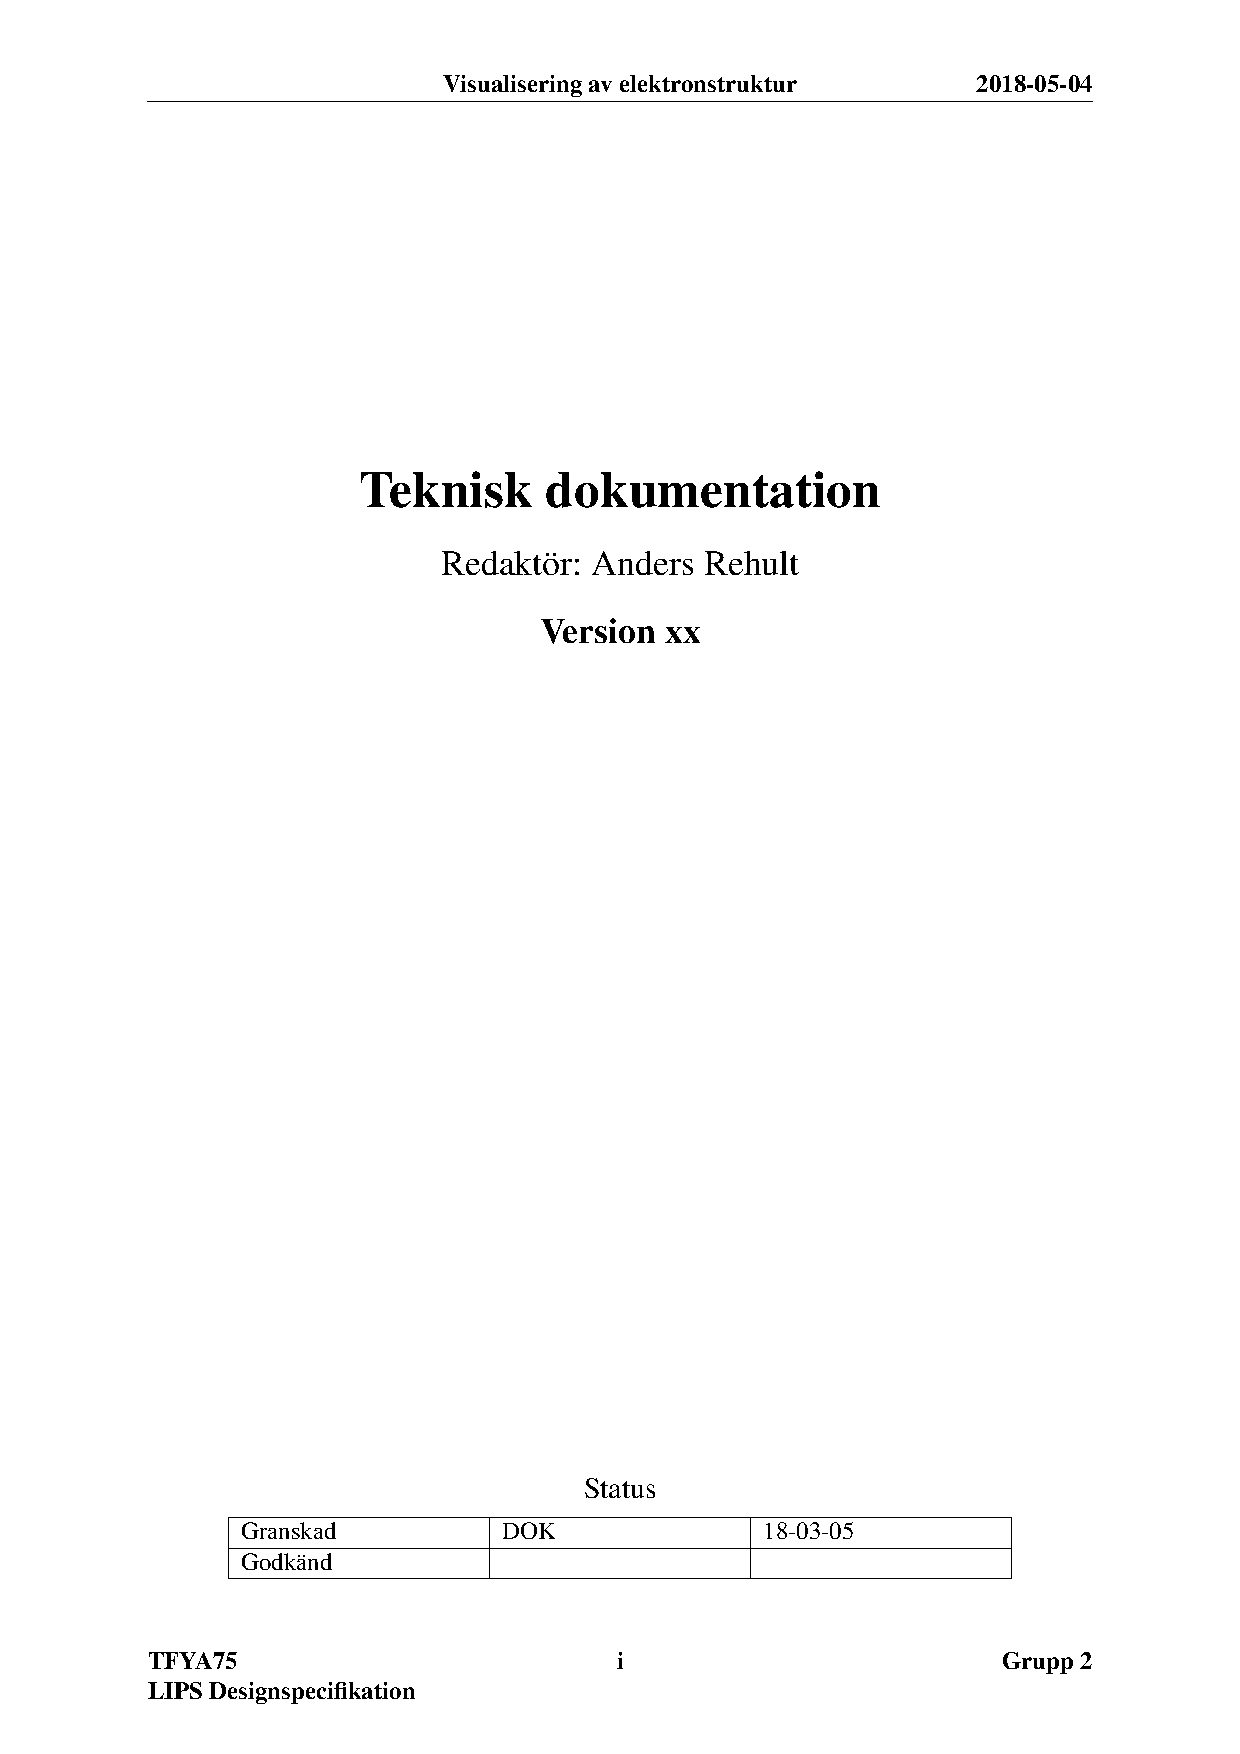
\includepdf[pages={1},pagecommand=\section{Teknisk dokumentation}\label{appendix:teknisk-dokumentation}\thispagestyle{empty}]{tekdok.pdf}
\includepdf[pages={2-}]{tekdok.pdf}

\end{appendices}

\end{document} 
